\documentclass[twocolumn]{bmcart}% uncomment this for twocolumn layout and comment line below
%%% Load packages
%\documentclass[doublespacing,twocolumn]{bmcart}% uncomment this for twocolumn layout and comment line below
%%% Load packages
\usepackage{amsthm,amsmath}
\RequirePackage[authoryear]{natbib}% uncomment this for author-year bibliography
\RequirePackage{hyperref}
\usepackage[utf8]{inputenc} %unicode support
\startlocaldefs
\endlocaldefs
\usepackage{graphicx}
%% increasing table spacing
\renewcommand{\arraystretch}{1.3}
% href 
\usepackage{cuted,tcolorbox}
\usepackage{caption}
\usepackage{multicol}
\usepackage{array}
\usepackage{hanging}
\usepackage{hyperref}
\hypersetup{
    bookmarks=false,         % show bookmarks bar?
    unicode=false,          % non-Latin characters in AcrobatÕs bookmarks
    pdftoolbar=false,        % show AcrobatÕs toolbar?
    pdfmenubar=true,        % show AcrobatÕs menu?
    pdffitwindow=false,     % window fit to page when opened
    pdfstartview={FitH},    % fits the width of the page to the window
    pdftitle={},    % title
    pdfauthor={},     % author
    pdfsubject={},   % subject of the document
    pdfcreator={},   % creator of the document
    pdfproducer={}, % producer of the document
    pdfkeywords={}, % list of keywords
    pdfnewwindow=true,      % links in new window
    colorlinks=true,       % false: boxed links; true: colored links
    linkcolor=black,          % color of internal links (change box color with linkbordercolor)
    citecolor=black,        % color of links to bibliography
    filecolor=black,      % color of file links
    urlcolor=black           % color of external links
}
%% fighting float spacing
\renewcommand{\topfraction}{.9}
\renewcommand{\bottomfraction}{.9}
\renewcommand{\textfraction}{0.1}
\renewcommand{\dbltopfraction}{.9}
\renewcommand{\dblfloatpagefraction}{.9}
\renewcommand{\floatpagefraction}{0}
\setcounter{topnumber}{9}

\setcounter{bottomnumber}{9}
\setcounter{totalnumber}{10}
\setcounter{dbltopnumber}{9}
\bibliographystyle{agsm}
\setcitestyle{authoryear,open={(},close={)}}
\usepackage{har2nat}
\begin{document}
\begin{frontmatter}
\begin{fmbox}
%\dochead{Opinion}

%%%%%%%%%%%%%%%%%%%%%%%%%%%%%%%%%%%%%%%%%%%%%%
%%                                          %%
%% Enter the title of your article here     %%
%%                                          %%
%%%%%%%%%%%%%%%%%%%%%%%%%%%%%%%%%%%%%%%%%%%%%%

\title{On the origin and structure of haplotype blocks}

%%%%%%%%%%%%%%%%%%%%%%%%%%%%%%%%%%%%%%%%%%%%%%
%%                                          %%
%% Enter the authors here                   %%
%%                                          %%
%% Specify information, if available,       %%
%% in the form:                             %%
%%   <key>={<id1>,<id2>}                    %%
%%   <key>=                                 %%
%% Comment or delete the keys which are     %%
%% not used. Repeat \author command as much %%
%% as required.                             %%
%%                                          %%
%%%%%%%%%%%%%%%%%%%%%%%%%%%%%%%%%%%%%%%%%%%%%%
\author[
  addressref={aff1,aff2,aff3}, 
   noteref={n1},% id's of addresses, e.g. {aff1,aff2}
%corref={aff1},                       % id of corresponding address, if any
% noteref={n1},                        % id's of article notes, if any
  email={daria.shipilina@ebc.uu.se}   % email address
]{\inits{D.}\fnm{Daria} \snm{Shipilina}}
\author[
  addressref={aff2}, 
   noteref={n1},% id's of addresses, e.g. {aff1,aff2}
%corref={aff1},                       % id of corresponding address, if any
% noteref={n1},                        % id's of article notes, if any
  email={arka.pal@ist.ac.at}   % email address
]{\inits{A.}\fnm{Arka} \snm{Pal}}
\author[
  addressref={aff2}, 
   noteref={n1},% id's of addresses, e.g. {aff1,aff2}
%corref={aff1},                       % id of corresponding address, if any
% noteref={n1},                        % id's of article notes, if any
  email={sean.stankowski@ist.ac.at}   % email address
]{\inits{S.}\fnm{Sean} \snm{Stankowski}}
\author[
  addressref={aff4}, 
% id's of addresses, e.g. {aff1,aff2}
%corref={aff1},                       % id of corresponding address, if any
% noteref={n1},                        % id's of article notes, if any
  email={frank.chan@tue.mpg.de}   % email address
]{\inits{Y.F.}\fnm{Yingguang Frank} \snm{Chan}}
\author[
  addressref={aff2}, 
% id's of addresses, e.g. {aff1,aff2}
%corref={aff1},                       % id of corresponding address, if any
% noteref={n1},                        % id's of article notes, if any
  email={nick.barton@ist.ac.at}   % email address
]{\inits{N.}\fnm{Nicholas H.} \snm{Barton}}


\address[id=aff1]{%                           % unique id
  \orgdiv{Evolutionary Biology Program, Department of Ecology and Genetics},           
  \orgname{Uppsala University},           
 % \street{Norbyvägen 18D},
  \postcode{75236}
  \city{Uppsala},                              % city
  \cny{Sweden}                                    % country
}
\address[id=aff2]{
%  \orgdiv{Institute of Biology},
  \orgname{Institute of Science and Technology Austria},
   %\street{Thunbergsvägen 2},
  \postcode{75236},
  \city{Klosterneuburg},                              % city
  \cny{Austria } 
}
\address[id=aff3]{
%  \orgdiv{Institute of Biology},
  \orgname{Swedish Collegium for Advanced Study},
   \street{Thunbergsvägen 2},
  \postcode{75236},
  \city{Uppsala},                              % city
  \cny{Sweden} 
}
\address[id=aff4]{
%  \orgdiv{Institute of Biology},
  \orgname{Friedrich Miescher Laboratory of the Max Planck Society},
   \street{Thunbergsvägen 2},
  \postcode{72076},
  \city{Tübingen},                              % city
  \cny{Germany} 
}


%%%%%%%%%%%%%%%%%%%%%%%%%%%%%%%%%%%%%%%%%%%%%%
%%                                          %%
%% Enter short notes here                   %%
%%                                          %%
%% Short notes will be after addresses      %%
%% on first page.                           %%
%%                                          %%
%%%%%%%%%%%%%%%%%%%%%%%%%%%%%%%%%%%%%%%%%%%%%%


\begin{artnotes}
%\note{Sample of title note}     % note to the article
\note[id=n1]{Equal contributor} % note, connected to author
\end{artnotes}

\end{fmbox}% comment this for two column layout

%%%%%%%%%%%%%%%%%%%%%%%%%%%%%%%%%%%%%%%%%%%%%%%
%%                                           %%
%% The Abstract begins here                  %%
%%                                           %%
%% Please refer to the Instructions for      %%
%% authors on https://www.biomedcentral.com/ %%
%% and include the section headings          %%
%% accordingly for your article type.        %%
%%                                           %%
%%%%%%%%%%%%%%%%%%%%%%%%%%%%%%%%%%%%%%%%%%%%%%%
\begin{abstractbox}

%\begin{abstract} % abstract
%\justifying
The term “haplotype block” is commonly used in the developing field of haplotype-based inference methods. We argue that the term should be defined based on the structure of the Ancestral Recombination Graph (ARG), which contains complete information on the ancestry of a sample. We use simulated examples to demonstrate key features of the relation between haplotype blocks and ancestral structure, emphasising the stochasticity of the processes that generate them. Even the simplest cases of neutrality or of a “hard” selective sweep produce a rich structure, often missed by commonly used statistics. We highlight a number of novel methods for inferring haplotype structure, based on the full ARG, or on a sequence of trees, and illustrate how they can be used to define haplotype blocks using an empirical dataset. While the arrival of computationally efficient methods makes it possible to apply these concepts broadly, existing and new methods could include tools for the identification and explore haplotype blocks, as we define them. Understanding and applying the concept of the haplotype block will be essential to fully exploit long and linked-read sequencing technologies.
%\parttitle{First part title} %if any
%Text for this section.

%\parttitle{Second part title} %if any
%
%Text for this section.
%\end{abstractbox}


%%%%%%%%%%%%%%%%%%%%%%%%%%%%%%%%%%%%%%%%%%%%%%
%%                                          %%
%% The keywords begin here                  %%
%%                                          %%
%% Put each keyword in separate \kwd{}.     %%
%%                                          %%
%%%%%%%%%%%%%%%%%%%%%%%%%%%%%%%%%%%%%%%%%%%%%%

\begin{keyword}
\kwd{haplotype block}
%\kwd{\emph{Vanessa cardui}}
%\kwd{effective population size}
\kwd{ancestral recombination graph}
%\kwd{insect migration} 
\kwd{haplotype-based methods}
\kwd{coalescent} 
\end{keyword}

% MSC classifications codes, if any
%\begin{keyword}[class=AMS]
%\kwd[Primary ]{}
%\kwd{}
%\kwd[; secondary ]{}
%\end{keyword}

\end{abstractbox}
%
%\end{fmbox}% uncomment this for two column layout

\end{frontmatter}

%%%%%%%%%%%%%%%%%%%%%%%%%%%%%%%%%%%%%%%%%%%%%%%%
%%                                            %%
%% The Main Body begins here                  %%
%%                                            %%
%% Please refer to the instructions for       %%
%% authors on:                                %%
%% https://www.biomedcentral.com/getpublished %%
%% and include the section headings           %%
%% accordingly for your article type.         %%
%%                                            %%
%% See the Results and Discussion section     %%
%% for details on how to create sub-sections  %%
%%                                            %%
%% use \cite{...} to cite references          %%
%%  \cite{koon} and                           %%
%%  \cite{oreg,khar,zvai,xjon,schn,pond}      %%
%%                                            %%
%%%%%%%%%%%%%%%%%%%%%%%%%%%%%%%%%%%%%%%%%%%%%%%%

%%%%%%%%%%%%%%%%%%%%%%%%% start of article main body
% <put your article body there>

%%%%%%%%%%%%%%%%
%% Background %%
%%
\section*{Introduction}

One of the breakthroughs of long and linked-read sequencing technologies is the emergence of new methods for obtaining reliable haplotype information for large data sets (Meier et al., 2021). Although most studies of genome-wide variation still focus on SNP data, we are approaching the stage where population-scale haplotype information will be widely available for organisms across the tree of life. In light of this shift from site-based to haplotype-based inference, this article considers one of the fundamental concepts for haplotype-based inference—the definition of the haplotype block.

“Haplotype” and “haplotype block” are widely used terms in evolutionary genetics, and have increased in importance across many disciplines (Delaneau et al., 2019; International HapMap Consortium, 2005; Leitwein et al., 2020). An important, but often overlooked fact, is that populations evolve through changing frequencies of blocks of the genome, and not individual sites. Therefore, we should be most interested in understanding the trajectories of the underlying haplotypes, yet these are often obscured at the level of SNPs (Castro et al., 2019; Clark, 2004). Thus, disentangling the evolutionary history underlying genomic patterns can be challenging using solely site-based statistics. For example, while whole-genome scans for signatures of selection can reveal individual SNPs associated with fitness differences (Poelstra et al., 2014; Tavares et al., 2018), it is extremely difficult to pinpoint the causal variants (Burri, 2017; Grossman et al., 2010; Ravinet et al., 2017; Rockman, 2012; Stankowski et al., 2019; Tavares et al., 2018; Wolf \& Ellegren, 2017). As another example, shifts in polygenic scores from genome-wide association studies (GWAS) can be misinterpreted as signals of selection, as opposed to artefacts of population structure (Berg et al., 2019; Novembre \& Barton, 2018; Sella \& Barton, 2019), which often leave clearer signatures in shared haplotype structure. 

Similarly, methods for estimating population density and gene flow struggle to distinguish among a virtually infinite number of possible population structures, made worse by assuming independence between SNPs, rather than haplotypes.  (Richardson et al., 2016; Sousa et al., 2011; Whitlock \& Mccauley, 1999). 

%width=\columnwidth,
%float, floatplacement=b,

By accounting for haplotype structure, it should be possible to make inferences more accurate and more efficient. Haplotypes carry information not only from mutation but also from recombination, which provides an additional ‘clock’ that can help to reveal past events (eg. Ralph \& Coop, 2013). Primarily for these reasons, there has been a steady increase in analytic methods that aim to infer haplotype structure from sequence data, or that exploit haplotype structure to make inferences about selection, gene flow, and population structure.

\begin{strip}
\begin{tcolorbox}[colback=blue!2!white,colframe=blue!60!black,title=Glossary,fontupper=\footnotesize\sffamily, before
skip=0pt,after skip=0pt]
\begin{tabular}{ m{4.2cm} m{10cm} } 
\textbf{Ancestral recombination graph (ARG)} & A graphical representation of the complete ancestry of a sample of genomes through a series of coalescence and recombination events. The ARG can be decomposed into a series of marginal trees that give the relationships between samples within each non-recombining region. \\
\textbf{Branch} & A part of a genealogical tree at a single locus, which connects two coalescence events \\
\textbf{Coalescence} & The merging of lineages in a common ancestor, as one traces lineages backward in time \\
\textbf{Edge} & A set of genomic regions that are the immediate ancestors of a specific coalescence event, and that are ancestral to a specific set of sampled genomes. An edge has two dimensions (generations x map length). Any SNP that fall on an edge will be shared by the set of descendant genomes, and only by those genomes \\
\textbf{Haplotype} & A haploid genotype. A diploid genotype consists of a pair of haplotypes. \\
\textbf{Haplotype block} & The set of genomic regions that descend from a particular edge in the ARG, which is defined by a unique coalescence event, and by the set of descendant samples \\
\textbf{Identity by descent (IBD)} & Segments of genome are identical by descent if they descend from the same common ancestor \\
\textbf{Lineage} & A chain of genes that descends from parent to offspring, or (tracing backwards) from offspring to parent. \\
\textbf{Linkage disequilibrium (LD)} & Non-random association of alleles at different loci \\
\textbf{Phasing} & The process of assigning alleles to the maternal and paternal chromosomes in a diploid individual. \\
\textbf{Time to most recent common ancestor (TMRCA)} & The time of the most recent coalescence event from which a focal set of samples descends
\end{tabular}\hfill
\end{tcolorbox}
\end{strip}

Although there has been significant progress toward the broader use of haplotype information in empirical studies (see overview in the Box 3), much of this lacks a unifying concept across fields spanning evolutionary and conservation genetics (Leitwein et al., 2020), human and medical genetics (Crawford \& Nickerson, 2005), and animal and plant breeding (Bhat et al., 2021; Mészáros et al., 2021). There is thus often little consensus on how haplotype blocks are defined, which complicates comparison of results. Worse, it may preclude insights that may otherwise arise from spotting commonalities that emerge under vastly different population parameters.

\begin{figure}
    %\centering
    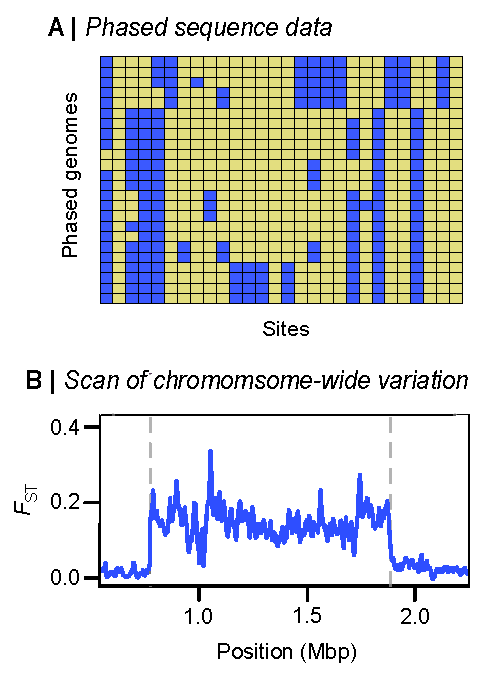
\includegraphics[width=0.89\linewidth]{Figure_1.pdf}
    \caption{\footnotesize{\textbf{Block-like patterns in empirical data}. (A) Block-like patterns in phased DNA sequences from Mimulus auranticus within the gene MaMyb2 (Stankowski \& Streisfeld, 2015). Rows show 24 individual haplotypes. Each column is a site with yellow and blue squares representing ancestral and derived sites, respectively. (B) An Fst scan across Helilconius chromosome 2 reveals a large plateau of differentiation on chromosome 2 between races of \textit{H. erato} (Meier et al., 2021). This large block-like pattern coincides with a chromosomal inversion, the boundaries of which are illustrated by the dashed line.}}
    \label{fig:1}
\end{figure}

Motivated by the arrival of powerful new datasets and analysis methods, the main goal of this paper is to examine the fundamental definition of the haplotype block. We propose a definition of haplotype block based on the full genealogy, represented by the Ancestral Recombination Graph (ARG). Using simulations of simple but general scenarios, we explore how the characteristics of haplotype blocks relate to the origin of the samples and segregating SNP variation. We then discuss how the proposed definition relates to practical inference methods and their applications in large-scale population studies. We consider how different methods make use of haplotype information and infer haplotype blocks, their underlying assumptions and respective limitations.

\section*{Defining haplotype blocks}
A haplotype has a clear definition: it is simply a haploid genotype (for example, the genotype of the sperm or egg). In contrast, the term “haplotype block" is used widely, but in many different ways (Al Bkhetan et al., 2019; Clark, 2004; International HapMap Consortium, 2005; Schwartz et al., 2003; Taliun et al., 2014; Zhang et al., 2002). Since haplotype structure arises through segregation and recombination, our understanding of “haplotype blocks” must depend on the processes of coalescence and recombination that generate it in the first place. With this in mind, we contrast alternative definitions, and settle on one, which is based on branches in the underlying genealogy.

In sequence data, we usually observe the diploid genotypes; resolving them into the two haploid genotypes is termed "phasing". With $n$ heterozygous sites, there are $2n$ possible pairs of haplotypes - more than a million with just $n = 20$. However, in real populations there are usually far fewer haplotypes, due to linkage disequilibrium (LD) across polymorphic sites, which produces strong haplotype structure. This allows “statistical phasing”, through which one reconciles diploid genotypes into the underlying haplotype pair (Browning \& Browning, 2011). Looking across individuals in larger genotype panels, the more frequent haplotypes often appear as stretches of shared, “banded” blocks of SNPs (Fig. 1A). This can be especially striking when different haplotypes become fixed across populations, which can produce block-like patterns in data even when individual haplotypes cannot be observed (Fig. 1B); in some cases, they have been referred to as ‘haploblocks’ (Todesco et al., 2020).

Whilst a block-like structure may be apparent within empirical genetic data, we argue here that there should be a more fundamental definition of haplotype block, based on the true ancestry of the sequences, independent of the mutations that generated observable SNPs. Thus, we separate the definition of haplotype blocks from the estimation of these blocks from actual data.

There have been previous attempts at defining haplotype blocks via the classical concept of identity by descent (Carmi et al., 2013; Hartl et al., 1997; Thompson, 2013). Imagine an initial population, where each founder genome is labelled by a different colour. At some later time, each region of the genome must derive from one or other founder, and so will appear as a mosaic of blocks of different colours, each corresponding to their ancestors. This naturally defines blocks that descend from a given set of founders (Fig. 2). Fisher (1954) showed that the junctions between IBD blocks segregate like Mendelian variants, and used this idea to understand the distribution of runs of homozygosity.

In artificial populations, we can now sequence the founders, and thus directly observe blocks defined in this way (Lundberg et al., 2017; Otte \& Schlötterer, 2021; Wallberg et al., 2017). Moreover, if we disregard new mutations, the evolutionary processes subsequent to the founding of the population are entirely described by the block structure. Identity-by-descent is usually defined with respect to a specific ancestral reference population. However, for natural populations, there is no obvious reference population, so the block structure will vary depending on our arbitrary choice of founders at an arbitrary time point (Figure 2); this makes the common practice of representing contemporary samples by admixture between well-mixed founder populations questionable (e.g. STRUCTURE; Pritchard et al.).

\begin{figure*}
    %\centering
    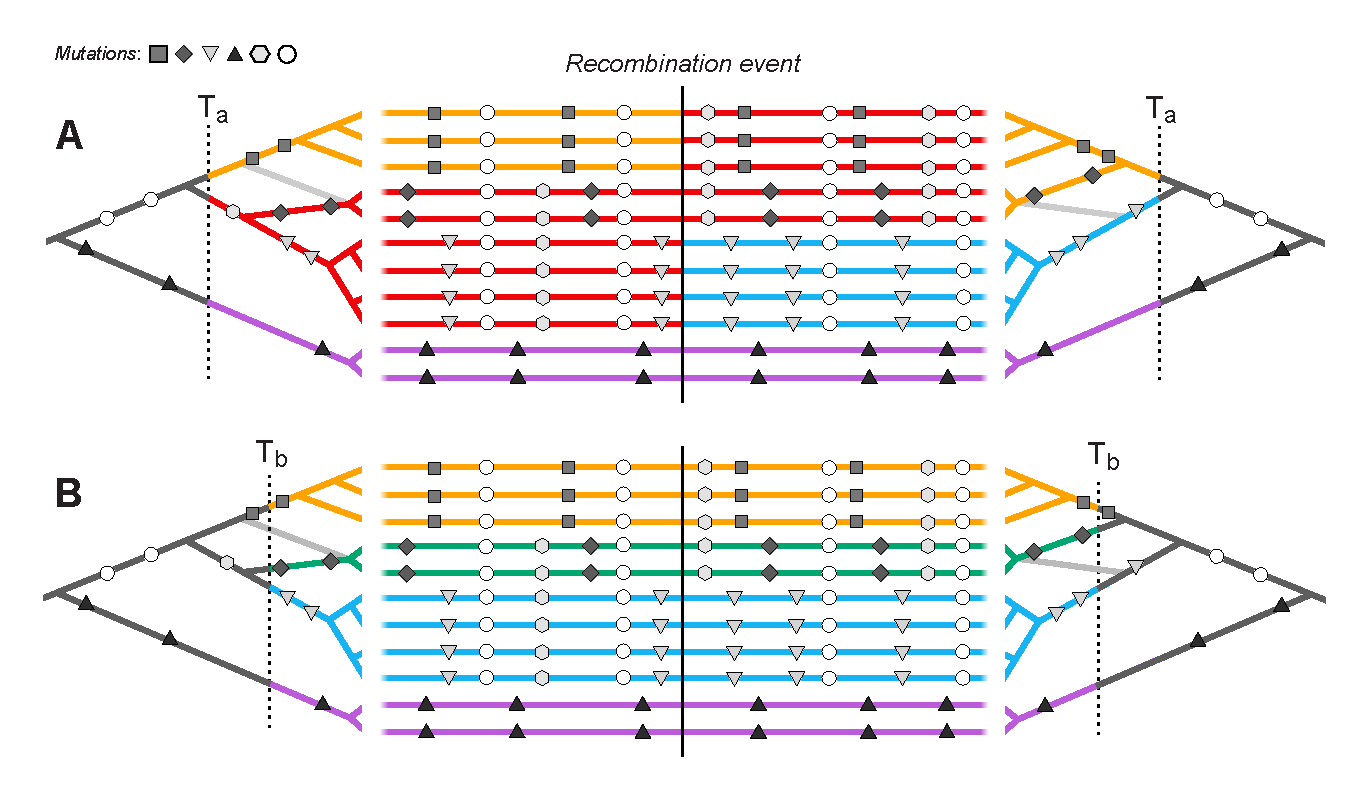
\includegraphics[width=0.89\textwidth]{Fig_2.pdf}
    \caption{\footnotesize{\textbf{Haplotype blocks defined through identity by descent (IBD)}. Panels A and B show the same 11 hypothetical DNA sequences depicted as horizontal lines. The trees on the left and right sides show the genealogy for the set of sequences on either side of a recombination event (indicated by the vertical black line); the light grey branch in both trees shows how the effect of recombination changes the structure of the genealogy on either side. Mutations are shown as symbols that correspond to the branches upon which they arose. Under the IBD definition, haplotype blocks can be defined based on DNA segments that derive from a given set of ancestors, shown here by the coloured sections of branch and DNA sequence. The only difference between panels A and B is that these ancestors are defined at two different arbitrary time points, Ta and Tb, yielding different haplotype structure.}}
    \label{fig:2}
\end{figure*}

To eliminate this subjectivity, we will base our definition of ‘haplotype block’ on the full ancestry of the sampled genomes, namely, on the ancestral recombination graph (ARG) (Hudson, 1983). The ARG consists of the segments of past genomes that are ancestral to our sample; looking back in time, it is generated by a series of coalescence events that join lineages and of recombination events that split lineages (Box 1). We emphasise that these are real events: coalescence occurs when an actual individual leaves two or more offspring that are each ancestral to our sample, and recombination occurs between the two haploid parent genomes during meiosis in an ancestral individual. Together, these processes define the ARG (Fig. B1). \\
In large populations, and over long timescales, the ARG is approximated by the coalescent with recombination; in the simplest case, the rate of coalescence is the inverse of the effective (haploid) population size, and the rate of recombination is just the rate of crossover (Hudson 1990, Griffiths \& Marjoram 1997). Importantly, the coalescent does not describe the entire genealogical relationship of the entire population. Rather, it only summarises how the subset of sampled individuals are related to each other. Spatial and genetic structure can also be included: ancestral lineages carry a particular set of selected alleles (i.e., a particular genetic background), and are at a particular spatial location. Tracing back in time, lineages move between backgrounds by recombination, and between locations by migration.

Informed by the ARG, we could define a haplotype block as a contiguous region of the genome in which all sites share the same genealogy. That is, we could decompose the ARG into marginal trees, each spanning a short region of genome. However, adjacent genealogies differ by a single recombination event, and so blocks defined in this way will be vanishingly small (especially with large samples) and will usually differ trivially (see A in Fig. 3 and Fig. B1A). Moreover, as samples get larger, blocks defined this way will become so small as to be impractical.

Instead, we define a haplotype block as the set of genomic regions that descend from a particular edge in the ARG which is defined by a unique coalescence event, and by the set of descendant samples.  Before elaborating on this definition, we clarify our terminology (see Glossary).  Consistent with the literature, we continue to use “haplotype block” to refer to a region of genome with a shared pattern of ancestry, without forcing a precise definition. By “branch”, we refer to a lineage on a genealogical tree that connects two coalescence events, or a sampled gene with a coalescence.  By “edge”, we refer to the extension of a branch along the genome.  Thus, a branch is one dimensional, with length measured in generations, whilst an edge is two-dimensional, with dimensions measured in generations as we trace back through time, and in Morgans as we trace along the genome.  An edge is associated with a specific coalescence event, and also with a specific set of descendant samples.

\begin{strip}
\begin{tcolorbox}[
  colback=blue!1!white,width=\columnwidth,colframe=blue!50!black,title= Box 1: Ancestral Recombination Graph (ARG),width=6.7in]
  
  \begin{multicols}{2}
\small{The ARG describes the complete ancestry of a sample of genomes through a series of real coalescence and recombination events (Griffiths \& Marjoram, 1997; Hudson, 1983). At any given site on the genome, the relationship can be described through a genealogy (Kingman, 1982); all contemporary samples coalesce and eventually trace back to one single ancestor. Moving along the genome, the relationship inevitably changes due to recombination. This leads to a series of observable genealogies along the genome (Fig B1A), which are embedded in a single structure - the ARG (Fig B1B). \\

The full ARG (Fig B1B) is a graph structure that depicts individuals (both ancestral and extant), lineage relationships in time. Each node in the ARG represents a real coalescence or recombination event, whilst edges represent the ancestry of a particular genomic segment, along a genetic lineage (depicted by coloured/grey segment for inherited/non-inherited genetic material in Fig B1B). Altogether, an ARG describes the entire ancestral history - each recombination and each coalescence event, which imply the genealogy for each non-recombined genomic block. Crucially, the ARG describes ancestry but not allelic state, so is independent of all the mutations that lead to the observed polymorphism in the present sample.\\

It is important to note that the full ARG (Fig B1B) contains more information than the series of tree sequences along the genome (Fig B1A). First, a series of tree sequences lack information on the timing of recombination events, unless these are separately stored. Second, while some recombination events lead to observable changes in genealogical trees, others might not. Figure B1A depicts such cases - some recombination events might not change the tree topologies at all (trees ii and iv are exactly the same), whereas others might only lead to temporal changes in coalescence nodes (tree $i$ differs from trees $ii$ and $iv$ by 1 node position, but all have the same topology). Therefore, while there are 4 non-recombining genomic regions, there are only 2 unique tree topologies (trees $i$, $ii$ and $iv$ have the same topology) and 3 distinct trees (trees $ii$ and $iv$ are exactly the same). Some coalescence events can also be entirely invisible and not be represented in any of the individual trees – coalescence at $t_2$ in Fig B1B is not represented in the series of trees in Fig B1A. Furthermore, two disjunct blocks of the genome can be inherited from the same ancestor, so that a unique coalescence event (e.g. marked by * in Fig B1A) can generate disjunct blocks of ancestry. It should also be noted that although Fig B1 shows the inevitable coalescence of the whole genome into a single common ancestor, this typically takes an astronomically long time: each non-recombining region of the genome coalesces at various time points, and the single lineages ancestral to each region then take an extremely long time to coalesce in one common ancestor, in a process which is in principle unobservable.} \\

\begin{center}
    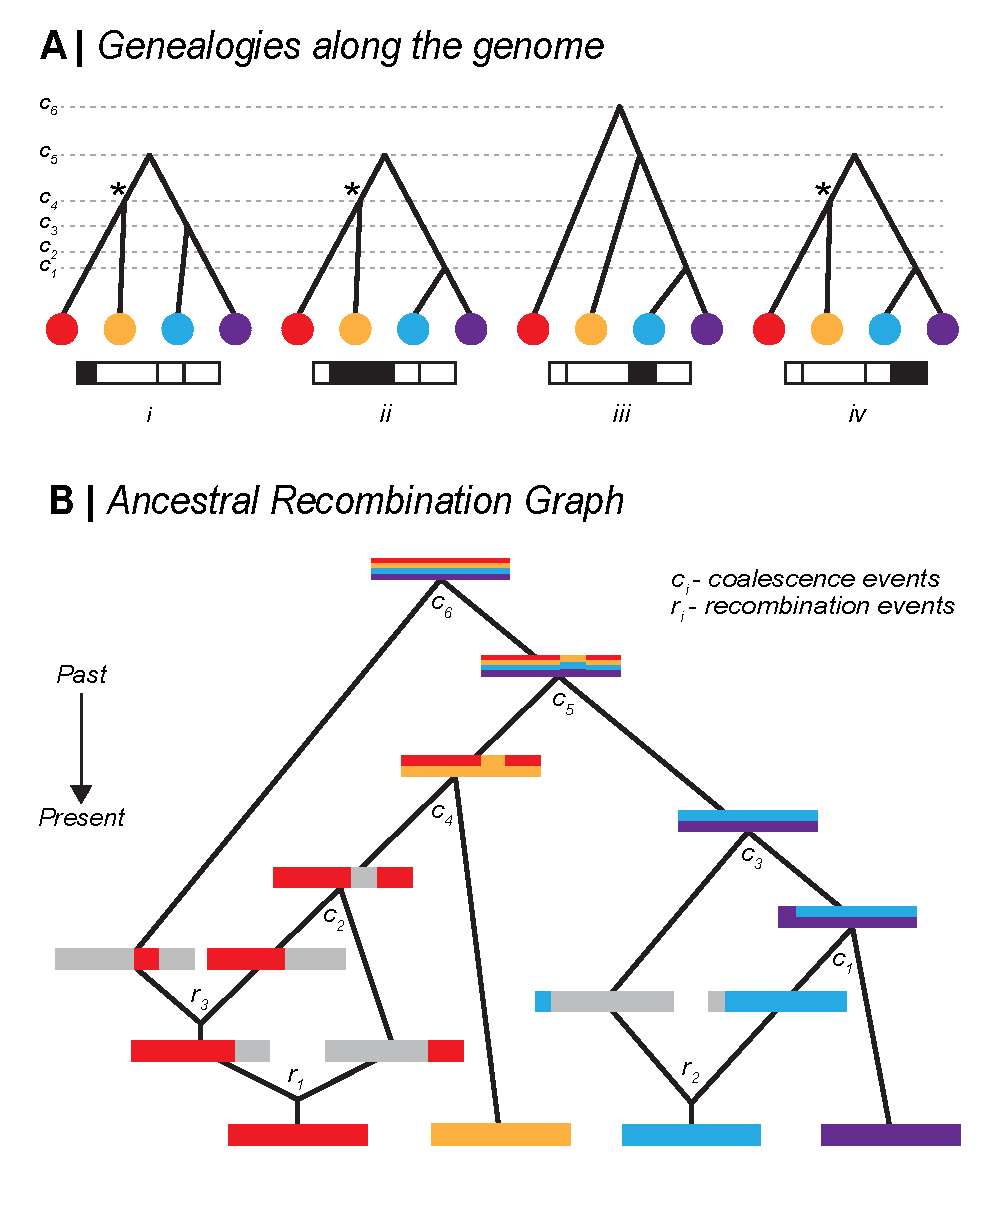
\includegraphics[width=0.99\linewidth]{Fig_B1.pdf}\end{center}
\captionof{figure}{
\footnotesize{\textbf{Relationship between Genealogies and the ARG}. (A) Genealogical trees along the genome, corresponding to the ARG - each tree describes the ancestral relationship for each of the 4 non-recombined regions. $c_1, c_2, ..., c_6$ denote time points for each coalescence event. Trees can either change, have the same topology, or marginally differ by only temporal positions of coalescence nodes. Asterisk (*) denotes a unique coalescence event that is ancestral to disjunct genomic regions. (B) Full representation of Ancestral Recombination Graph (ARG) - Tracing back ancestry of four genomes, there is either recombination splitting lineages or coalescence merging lineages. Inherited ancestral genomic regions are coloured corresponding to the contemporary genomes. Recombination is represented by splitting the genome into two; where grey denotes non-ancestral genomic region. Coalescence is represented by two genomes merging, with inherited genomic regions denoted by mixed colours. There are 3 recombination and 6 coalescence events in the full ancestral history of the four genomes. $c_1, c_2, ..., c_6$ denotes time points for each coalescence event. $r_1, r_2, r_3$ denotes time points for each recombination event. }  
\label{fig:B1}}

\small{Since the ARG contains full information about the genealogy of the sample, it is in theory sufficient to infer any evolutionary process: the ARG necessarily gives more information than commonly used statistics like SFS, $F_st$, EHH, which are low-dimensional summaries of the ARG (Ralph et al., 2020). Therefore, the ARG should serve as the foundation for developing new methodologies. However, we note that whilst the ARG is a sufficient statistic, it remains an open question how much the extra information it gives can improve inference: the intrinsic variability of the evolutionary process sets a bound on the accuracy of our inferences.}
\end{multicols}

\end{tcolorbox}
\end{strip}

This definition means that haplotype blocks exist completely independent of SNPs that may happen to arise on a given edge. However, if mutations have occurred, haplotype blocks will be associated with the set of derived SNP alleles that arise on the focal edge that just precedes the coalescence event. In other words, the set of haplotypes descending from this edge are distinct from all other sampled haplotypes in that they—and only they—share the set of SNPs occurring in the common stem lineage. If enough SNPs happen to arise on an edge, the haplotype block is revealed directly by these shared SNPs.

\section*{Implications of the definition}
We next elaborate on the definition and illustrate the relationships between genealogies, SNPs and haplotype blocks using example simulations (a neutral scenario and a selective sweep; supplement 1). The simulation uses the standard coalescent (Wakeley, 2009) to generate the ancestral recombination graph, thereby tracking the ancestors of a sample of genomes back through time, until all ancestral genomes are ancestors to the whole sample. It assumes a Wright-Fisher model with a constant population size $2N$ haploid genomes. A region of the genome of map length R is followed, with the selected locus at the leftmost point (i.e., at 0). For simplicity, we allow at most one crossover per generation, with probability R; we simulate $R << 1$, so this is close to the case with no interference between crossovers. The simulation can be conditioned on a selective sweep, which is defined by the numbers of copies of the favourable allele in the population. Once the ARG is constructed, genealogies along the genome can be followed, and edges can be identified. Neutral SNPs can be added, assuming infinite-sites mutation; each SNP is associated with an edge in the ARG (more details on simulations in Supplement 1)

\begin{figure*}[h]
    %\centering
    \includegraphics[width=0.69\textwidth]{Fig_3.pdf}
    \caption{\footnotesize{\textbf{The relationship between trees (top), SNPs (middle), and haplotype blocks (bottom) in the neutral simulation (see main text for simulation details)}. The ARG has been decomposed into marginal trees (a - o) to show all of the unique topologies that coincide with the genomic spans shown in the central panel (also labelled a - o). The branches for each tree are coloured according to the 8 edges in the ARG that we chose to focus on (also labelled i – vii).  (A) Two neighbouring topologies that differ only slightly due to recombination. (B) An example of two trees ($k_1$ and $k_2$) that have the same topologies but different lengths. The central panel shows 10 haploid genomes (labelled 1 – 10, top to bottom, coinciding with the tips of the trees). The SNPs that arose on the 8 focal edges are indicated by the coloured circles. The lower panel (Blocks) shows the haplotype blocks for each edge. The coloured block in each panel is the focal edge, with the other 7 blocks shown in grey. The mutations shown in the central panel are projected onto each block (black circles) at the genomic location and time that they arose. They are also plotted onto the genomic position axis to make the connection with the centre panel mode explicit. Similarly, the numbers at the bottom right corner indicate which DNA sequences the mutations are associated with. (C \& D) Examples of regions of blocks that, by chance, are not revealed by mutations arising on the corresponding edge. (E \& F) Examples of nested haplotype blocks, where the ancestral block is highlighted with a coloured outline.}}
    \label{fig:2}
\end{figure*}

Figure 3 shows the relationship between trees, SNPs and haplotype blocks arising from the first simulation - a neutral example capturing the ancestry of 10 genomes, sampled from a population of 100 haploid individuals, across 10cM of the genetic map (Supplement 1). SNPs were generated by infinite-sites mutation with mutation at twice the rate of recombination. Despite the relatively short map and few individuals, this simulation is general because time and map distance both scale with population size (Hudson, 1990). Thus, the 268 generations taken for every part of the simulated genome to coalesce in a single common ancestor scales to $2.68N$, and the simulated map length scales to $10/N$, where $N$ is the effective size. Thus rescaled, this simulation shows a generic pattern, independent of population size. 

The central panel of Fig. 3 (middle panel, ‘SNPs’) shows the distribution of SNPs on the ten sampled genomes, coloured according to the edge on which they arose (we illustrate 8 edges with four or more SNPs each, out of 55 unique edges). Recombination events (24 total) have divided the genome into 34 intervals due to nested recombination events (which split longer genealogies into nesting, inner intervals; Fig. 3; top panel, ‘Trees’). This illustrates how recombination modifies the coalescent (also see Fig. B1 for schematic representation of the process). The ARG can be decomposed into 24 unique marginal trees, some of which show an identical topology and differ only in timing (branch length); thus 15 distinct topologies are shown in the top panel of Fig. 3 (trees and corresponding regions on the genome labelled $a - o$; compare $k_1$ and $k_2$ for an example of genealogies that share topology but differ in depth, B in Fig. 3).  

The coloured blocks shown in the lower panel of Fig. 3 (‘Blocks’) illustrate the extent of each edge along the genome, and through time. The mutations arising on each branch are projected onto the edge at the time and genomic position that they arise. The number of SNPs arising on each edge is Poisson distributed, with the expected number proportional to the area of the edge; this area is the sum of the genomic lengths that each ancestor carries, and that is ancestral to the coalescence event that defines the branch. We emphasise that the visualised colour blocks represent true genealogies—and are independent from mutations. Because mutation, or SNP occurrence, is a random process, some regions may not carry any informative SNPs. For example, though edge $i$ (light blue) is relatively well covered by 9 SNPs, none of them fall in the shallow region to the left (C in Fig. 3). Similarly, edge $ii$ has only 6 SNPs, none of which happen to fall in the rightmost region (D). Ultimately, the distribution of SNPs sets a limit on what can be inferred from sequence data; edges without mutations will be invisible to us, and our ability to infer the length of a block depends entirely on where mutations happen to fall. 

Each edge coincides with a specific coalescence event that brings together a specific set of lineages: in other words, edges are defined by both the coalescence event and the set of lineages. A single coalescence, i.e., a single ancestor, may generate multiple edges: the two genomes that come together in that event may carry a mosaic of ancestral material, in several combinations. A single coalescence event may even generate an edge that carries disjunct segments of the genome. This did not occur for any of the focal edges in the example of Fig. 3, but is not unlikely, especially in a selective sweep. Conversely, two different coalescence events may happen to bring together the same sets of lineages; their edges could only be distinguished through the different times of coalescence.

Because each edge is generated by a single coalescence, it begins at the same time across its whole extent (so, edges are bounded by a horizontal line at their base in the lower panel of Fig. 3). Recombination events split distal segments, thus limiting the span of the block along the map. Tracing back in time, edges must end in coalescence events that combine them with yet more descendants. These may occur at different times if there have been recombination events, so that the upper boundary is typically ragged.

\begin{figure*}
    %\centering
    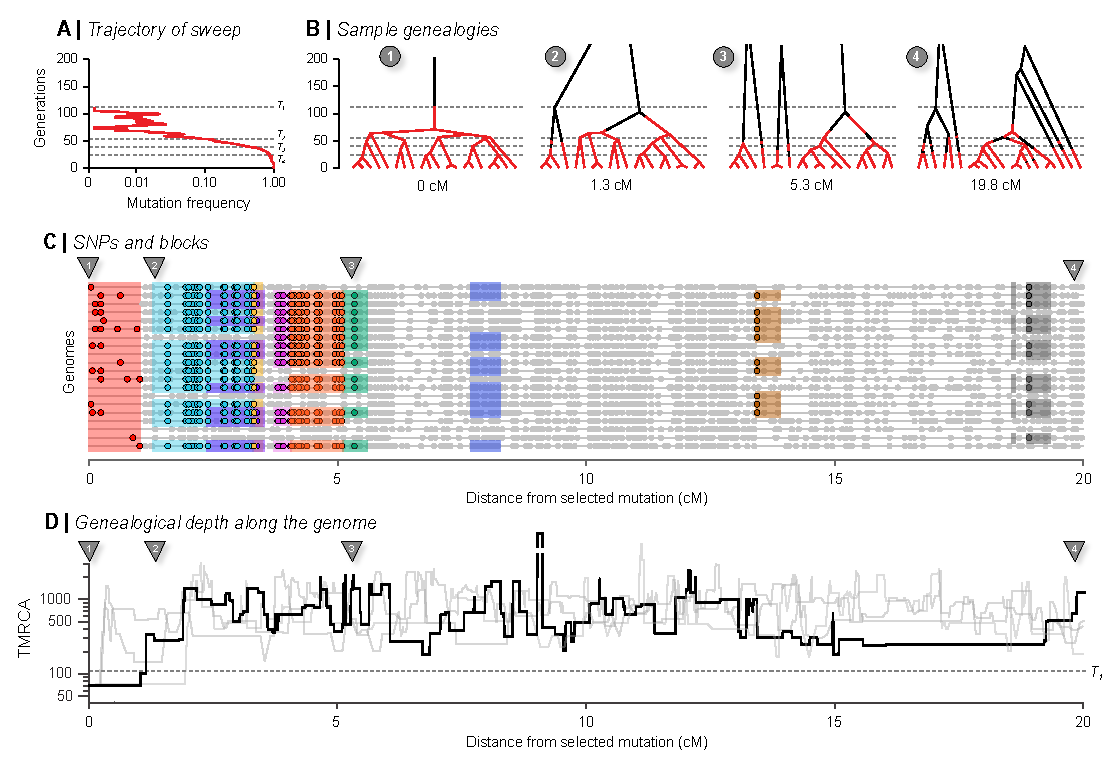
\includegraphics[width=0.79\textwidth]{Fig_4.pdf}
    \caption{\footnotesize{\textbf{The effects of a recent selective sweep on linked genealogies}. (A) A mutation with advantage 10\% arose in a population of 400 haploid individuals, and swept to fixation in 110 generations, at which time 20 genomes were sampled; 20cM of the genome is followed back in time, with the selected locus at the left.; dashed lines (T1 - T4) show times when the favoured allele was in 1 copy, at 10\%, at 50\%, and at 90\% (110, 53, 38, 22 generations back). (B) shows genealogies at positions 0, 1.3cM, 5.3cM, and 20cM, branches are coloured in red when on the fitter background, and black when on the ancestral background. Thus, changes in colour show recombination events that change the genomic background. Note that such events are unlikely when the allele is near fixation (i.e., at the base of the tree, below the lower dashed line), and conversely, become common whilst the allele is rare, simply because it will almost always meet with the opposite background. Before the mutation occurs (i.e., above the upper dashed line) lineages must either trace back to that mutation (top left) or recombine out into the ancestral background; thus, all lineages must appear black above the upper dashed line (110 generations back). Note that the disjunct branches in trees 2 - 4 all coalesce further back in time, but only 200 generations are shown for visibility. (C) shows SNPs along the 20 sampled genomes. The 9 of the most substantial branches are shown. (These have more than 8 descendants, formed by coalescence more recently than the sweeping mutation, and have areas $>0.5$). The red block at the left shows the region linked to the selected locus, which coalesces in a single common ancestor 69 generations back, just after the sweeping mutation arose. Grey dots show those SNPs that are not on these 9 highlighted branches. (D) shows the time back to the most recent common ancestry (TMRCA) along the genome, on a log scale. The bold line shows the example simulated above, whilst the three grey lines show replicates, generated conditional on the same sweep; the break in the line shows an area where the TMRCA extends further back than the extent of the y-axis. The dashed line across the plot corresponds to T1 in panel A.} }
    %\label{fig:2}
\end{figure*}

Haplotype blocks overlap in their genomic extent, since multiple lineages exist at any time more recent than the MRCA; this is shown by the overlapping 3-D blocks in Fig. 3 (‘Blocks’). Haplotype blocks will also overlap in the genome when edges are nested in the genealogy, giving rise to nested haplotype blocks. For example, edge ii (orange), which is ancestral to genomes 4 and 8 descends in the middle part of the genome from edge i (blue), which is ancestral to genomes 4, 7, 8 and 10. Thus, edge i is nested above block ii in Fig. 3 (see also F for another example of nested haplotype blocks). 

If we start at a particular site on the chromosome, and work along the genome, at some point an edge will be split by a recombination event. If the recombination occurs on the edge itself, the edge will persist, but most likely with a different depth. If the recombination event occurs outwith the lineages that descend from the focal coalescence, but coalesces into those lineages, then the set of descendants will be augmented, and the edge will end. Conversely, if the recombination event occurs amongst the descendant lineages, then some descendants will be lost, and the edge will again end. 

As we work out from a given locus, the incidence of recombination is proportional to the branch length, and so we expect that if a branch traces back deep into time, it will extend over a short region of the genome. Conversely, shallow branches will extend over a longer genomic span. This pattern is seen clearly in Fig. 3 (lower panel, "Blocks"), where edges consist of segments that are either deep and narrow, or shallow and wide. However, this relationship is not precisely inverse; if it were, edges would tend to have the same area, whether they were deep or shallow, and hence would carry similar numbers of SNPs. In fact, the distribution of areas of blocks is highly skewed, and so most SNPs are on a few deep branches (see discussion on branch depth in Supplement 1).

Note that under the coalescent process, large numbers of sampled lineages rapidly coalesce down to a few, which are then likely to trace back deep into the genealogy. Thus, in a given region of the genome a substantial fraction of SNPs will fall on long, deep, branches, whereas the tips of the genealogy will be hard to resolve. Moreover, in a large sample, it is unlikely that different coalescence events will bring together exactly the same set of lineages by chance, so that we can usually identify unique coalescence events as corresponding to unique sets of lineages. This is one reason why haplotype-based analyses can be particularly useful in disentangling genetic structure.

Figure 3 illustrates the simplest case of the standard coalescent with recombination. In reality, population structure and selection complicate genealogies. For example, in the island model, lineages either coalesce quickly within a deme, or escape to coalesce much further back in time. This exaggerates the tendency for genealogies to be dominated by a few long branches (Wakeley, 2009). Selective sweeps have a somewhat similar effect. In the classic case (Maynard Smith \& Haigh, 1974), all lineages at the selected locus coalesce in the individual that carries the favoured mutation. Moving out from this locus, recombination frees lineages to coalesce much further back.

Figure 4 illustrates such a selective sweep (Supplement 2). The sweep greatly reduces diversity around the selected locus, because all lineages must trace back to the successful mutation (Fig. 4B, 1). This region of complete coalescence is shown in red, but note that it contains some diversity, due to mutation subsequent to the sweep. As we move away from the selected locus, lineages recombine out onto the ancestral background, and coalesce with the rest of the genealogy much further back (Fig. 4B).  This process can be seen in the TMRCA (Fig. 4D), which jumps from a low value at the selected locus, through successive recombination events, back to a time that fluctuates around $4N_e=800$ generations, under the standard coalescent. However, the replicates in the lower panel show that there is considerable variation in this process, which sets a fundamental limit on our power to detect a sweep and estimate its properties.

At the selected locus, all lineages coalesce in the favoured mutation. Successive recombination events each free one or a few lineages from the new background, so that the exceptionally large and recent cluster gradually diminishes in size, until the genealogies follow a close to neutral distribution. Thus, edges with large numbers of descendants are associated with the sweep, and can be distinguished by the characteristic sets of SNPs that they carry; nine such edges are illustrated in Fig. 4C. 

We close this section by commenting on possible connections between our description of the ARG, and practical inference. Stern et al. (2019) propose a method that infers the allele frequency trajectory from the genealogy at the selected locus, which is assumed to be known.  The extent of the focal edge along the genetic map gives additional information, with a predicted constant rate of recombination out into the ancestral background, at a rate equal to the frequency of the ancestral allele.  Additional edges give more information: in particular, several lineages may coalescence early in the sweep, but then recombine out (e.g. the second genealogy in Fig. 4B). This generates multiple long branches, whose distribution depends on $4N_es$ (Barton, 1998).  There is considerable scope for using the extent of edges along the genome, as well as the genealogy at specific loci.

Nevertheless, we make two cautionary comments. First, there is considerable variability between different realisations, given the same trajectory (e.g. Fig. 4D) (i.e., the selective sweep itself is a stochastic process). Moreover, if the locus is identified from a genome-wide scan, ascertainment bias will distort the ARG: indeed, sequence variation around a neutral locus that experiences a sweep by chance may be indistinguishable from a genuinely selected locus.  This poses fundamental limits to our ability to estimate selection at a particular locus.  Second, sophisticated methods based on simple scenarios will be confounded by deviations from the model. For example, the extent of reduced diversity along the genome is the inverse of the time taken to reach high frequency - but that may be greatly increased by population structure. The visualisations that we develop here may have the greatest value in allowing us to check whether the fine structure of a candidate region is actually consistent with some simple model. It remains to be seen how far the rich information contained in the structure will help us improve our inferences.


\section*{The definition in practice}
Having defined haplotype blocks conceptually, we next consider the problem of inferring haplotype blocks from empirical datasets. Current sequencing and genotyping technologies make it straight-forward to identify SNPs or small insertions/deletions, but it remains non-trivial to connect these to the haplotypes in which they are embedded. For that reason, sophisticated algorithms have been developed for phasing, imputing genotypes and inferring genealogies (Browning \& Browning, 2009, 2013; Davies et al., 2016; Howie et al., 2011; Marchini et al., 2007). These tasks all engage different facets of the same problem, and rely to various extent on the haplotype structure. However, these methods tend to focus on phasing and stop short of inferring underlying haplotype structure and in particular the ARG, and haplotype blocks as we define them. In this section, we wish to focus on how haplotype blocks can be defined and visualised in practice. Given our ARG-based definition, we used ARGweaver (Rasmussen et al., 2014) to analyse an empirical dataset. We discuss other methods that use the ARG or approximations to it. We discuss the underlying assumptions of these methods and highlight where they could be extended to capture further information in light of our proposed definition of haplotype blocks as edges. Separately, in Box 2, we outline classes of simpler methods that use fixed genomic windows or genomic segments as a proxy for the haplotype block.

\begin{figure*}
    %\centering
    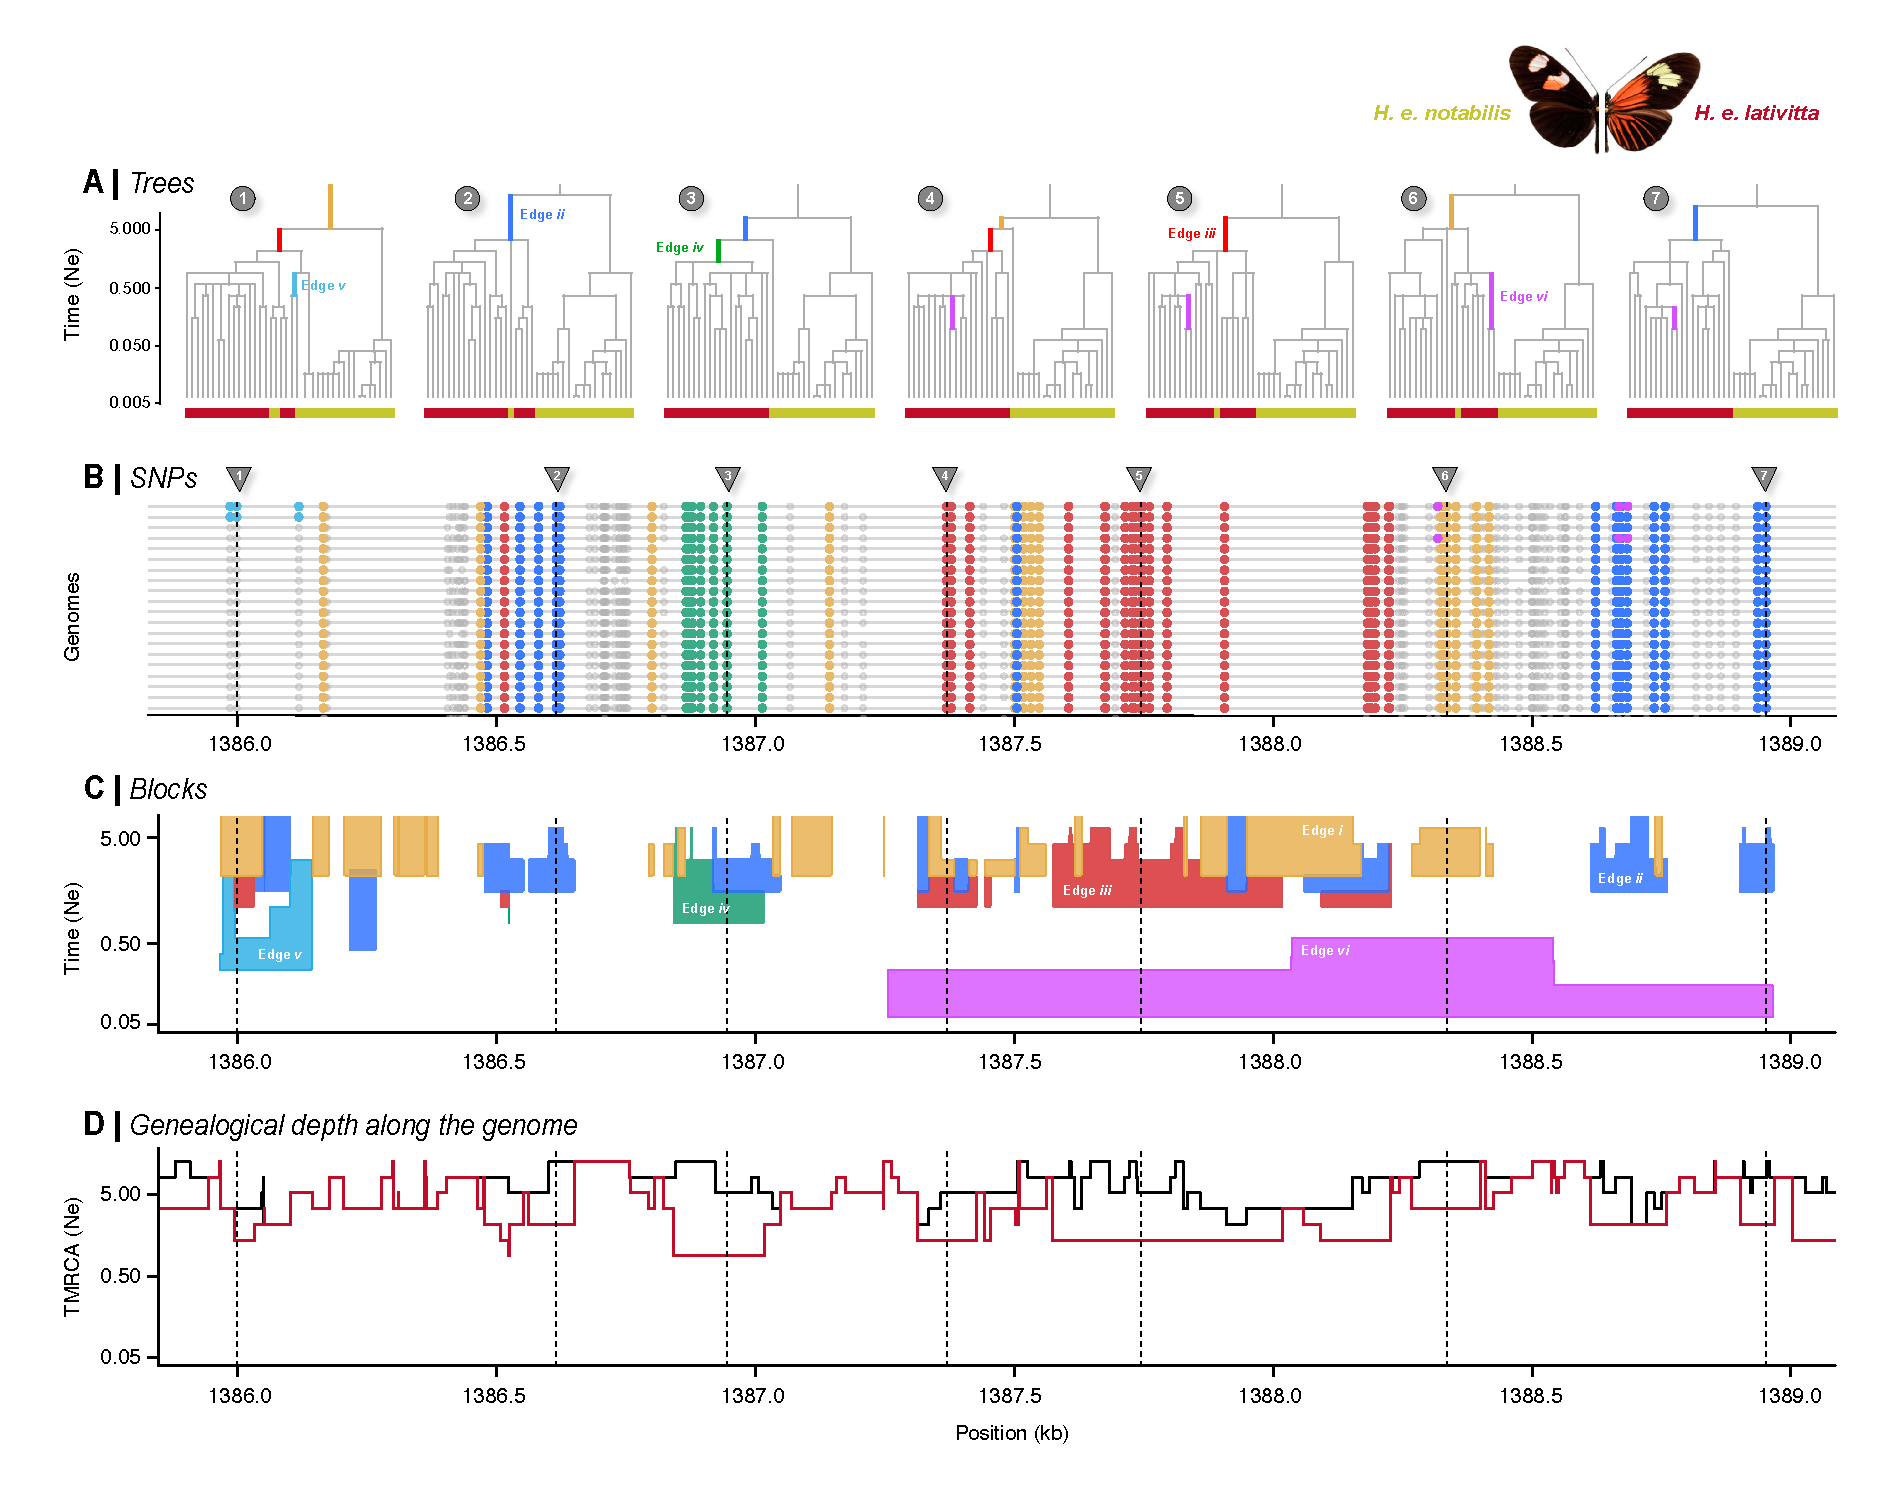
\includegraphics[width=0.89\textwidth]{Fig_5.pdf}
    \caption{\footnotesize{\textbf{Visualisation of haplotype blocks based on
application of ARGweaver to the \emph{optix} region of \emph{Helconius
erato} butterflies ($2n = 20$)}. (A) Genealogical trees at each
genomic point, marked by arrows and corresponding numbers. \emph{Red}
labels - \emph{H. e. lativitta} samples; \emph{Yellow} labels: \emph{H.
e. notabilis} samples. Branches on trees are coloured according to the
corresponding edges in \emph{C}. Both highland \emph{H. e. notabilis}
population ($2n = 20$) and lowland \emph{H .e. lativitta} ($2n = 20$)
are included in the analysis so that we can estimate the length of
branches that are ancestral to all \emph{H. e. lativitta} samples
($2n = 20$), however \emph{B,C,D} only exhibits features related to
H. e. lativitta population. (B) Genomic location of SNPs for all 20
\emph{H. e. lativitta} haploid samples. Out of a total of 137 SNPs, only
those that explain the 6 substantial edges are coloured accordingly.
Edges are defined as substantial if 3 or more SNPs occur on them. 2 out
of 6 edges (\emph{v} and \emph{vi}) are explained by doubleton SNPs,
whereas the rest are fixed within the \emph{H. e. lativitta} samples.
SNPs that do not appear on any significant edge are coloured grey if
they have higher allele frequency within the samples, white otherwise.
(C) Visualisation of haplotype blocks as edges similar to Figure 3 -
plotting blocks along the genomic (x-axis) and temporal span
(y-axis). Since edges always originate at a fixed coalescent time
point, the bottom line of the block is always smooth. The ragged tops of
the blocks denote the length of the edges interrupted by recombination
events. Note that edges can also be disjunct due to one or more samples
and recombining out and back into the same lineage. (D) 50-percentile
TMRCA estimates along the genome: black: total TMRCA to the all 40
samples, red : TMRCA to only \emph{H. e. lativitta} samples} }
    %\label{fig:2}
\end{figure*}

The full ARG contains all the information needed to apply the haplotype block definition to empirical datasets. Therefore, one could start by inferring the ARG (or even a sequence of genealogies along the genome) from a sample of sequences, identifying important edges on that ARG, and consequently the haplotype blocks that descend from those edges. ARGweaver (Rasmussen et al., 2014) and its extension ARGweaver-D (Hubisz et al., 2020) are among the most powerful tools for direct inference of ARG. One practical speed-up employed by ARGweaver is to discretize time, effectively making the ARG space finite by limiting recombination and coalescence events to discrete time points. Further, ARGweaver uses an approximate model, Sequentially Markov Coalescent (SMC; McVean \& Cardin 2005; extended by Marjoram and Wall 2006 (McVean \& Cardin, 2005) to sample from a distribution of ARG. While making inference more tractable, the SMC precludes the inference of disjunct blocks, because only one immediately prior state is considered as one moves along the genome. However, even with these key innovations, inference of the “full” ARG remains computationally expensive, making ARGweaver feasible for up to approximately 50 samples.

To illustrate our concept, we applied ARGweaver to infer the ARG from an empirical, phased dataset in \textit{Heliconius erato} butterflies. The dataset was generated by haplotagging, a technique for producing synthetic linked-read sequence data (Meier et al. 2021). We focus on the genomic region containing the gene \textit{optix}, where a selective sweep was previously inferred using site-based statistics (Fig S3, Supplementary Data 1). For comparison, we also sampled ARGs from a neutral background locus (Fig S3, Supplement 2). Figure 5 shows a focal region approximately 100 kbp 3’ from \textit{optix} that may correspond to a distal regulatory hub controlling the distinctive wing rays (“Ray” and “Dennis” elements, (Wallbank et al., 2016), possibly corresponding to obs132, LR1/2 and obs214, see Lewis et al., (2019)) at which all lowland \textit{H. e. lativitta} butterflies (red labels in Fig 5A) share a haplotype (Meier et al, 2021). To run ARGweaver, we used $r = 2.9\times10^{-9}$ and $N_e = 1.94 \times 10^{6}$ (calculated by estimating $\pi$ from the neutral region) and 30 discrete exponentially distributed time points (Fig S1). The key step for visualising haplotype blocks is identifying unique edges based on the sampled ARGs. We identified edges using custom scripts to parse marginal trees along the genome in order to identify branches
 that originate at a particular coalescent time-point (say, t1), and are ancestral to a fixed set of individuals (say, x1, x2, x3) (see Table S1, S2). This set of branches represents an edge that is defined by {t1}, {x1, x2, x3} and the trees that contain the above branches (see branches in Fig 5A coloured according to haplotype blocks as edges in Fig. 5C). Here, we chose to focus on the 6 edges that are supported by 3 or more SNPs (Fig 5B: SNPs; 5C: haplotype blocks as edges) (see Table S3 for a list of all edges supported by SNPs). We then visualised haplotype blocks based on these edges, including both their genomic span (i.e., the tree-spans along the genome containing the edge) and temporal span (length of each tree branch that constitutes the edge) (Fig 5C). 

We find a rich structure of haplotype blocks in the focal region. First, in regions of shallow coalescence, we see structured uninterrupted haplotype blocks that carry SNPs fixed in all \textit(H. e. lativitta} samples (Fig 5). For example, the shallowest coalescence region constitutes the uninterrupted haplotype block defined by edge iv, and is supported by 9 SNPs. Adjacent to edge iv, we find the largest haplotype block defined by edge iii and supported by 22 SNPs, which coincides with a putative selective sweep that was previously identified using the omega statistic (Wallbank et al., 2016; Lewis et al., 2019). Unlike edge iv (green), edge iii (red) exists as disjunct blocks separated primarily by recombination events that shifts the total coalescence within \textit{H. e. lativitta} samples to occur slightly further back in time (see Trees 3,4,5,6 for reference). Moving along in both directions from the central shallow TMRCA region, we observe other haplotype blocks, exhibiting different histories (originating deeper in the past) spanning as disjunct blocks along the entire genomic region and supported by fixed SNPs (edge i and ii). Although the SMC precludes ARGweaver from inferring disjunct coalescence events, disjunct blocks (especially, edge i) may be an artefact of the way we identify unique edges from the ARGweaver output, together with discretization of time points (in principle, they could be distinct coalescence events but are forced to coalesce at the same time). Moreover, these blocks can also stem from including the \textit{H. e. notabilis} population in our analysis (Trees 1, 2, 5, 6 has one or more \textit{H. e. notabilis} individual clustering together within the \textit{H. e. lativitta} population), and hence are present as nested blocks within edge iii and iv in the central regions of the shallowest coalescence. In future, it would be interesting to examine if additional evidence can suggest older, historical sweep events to explain the disjunction of these blocks, or whether they are simply remnant structures/signatures from other stochastic events. It is important to note that 4 out of the 6 substantial edges drawn here are supported by SNPs fixed within the \textit{H. e. lativitta} samples, and spans in disjunction (except edge iv) throughout the region. This is in agreement with theoretical expectations in a swept genomic region where uninterrupted edges are expected to exist with multiple SNPs supporting them (edge iv - 9 SNPs, iii - 22, ii - 16, i - 14). In addition to these 4 blocks, we also see more recent blocks with greater spans, explained by singletons (see Fig S7) and doubletons (edge v and vi in Fig 5). Edge vi specifically spans the furthest along the genome, since it is formed by a coalescent event between only two samples, suggesting that there has not been sufficient time for recombination to break it down. 

\begin{strip}
\begin{tcolorbox}[colback=blue!2!white,colframe=blue!50!black,title= Box 2: Population genetic methods that make use of haplotype information]
  \begin{multicols}{2}
\footnotesize{Many methods for inferring evolutionary processes make use of haplotype structure. These can be roughly grouped into three types based on their underlying paradigm: window-based methods, segment-based methods and tree-based methods. These methods vary in complexity from simple heuristics to full statistical treatments. Here we discuss window-based and segment-based methods, but we reserve our discussion of tree-based methods to the main text. \\

Of the three classes, window-based methods tend to be the simplest, and primarily operate across sets of individuals. In the simplest form, haplotypes are operationally defined as the set of alleles observed at the segregating sites within a predefined window of an arbitrary length, say, 50 SNPs or 100 kilobase. Ideally, window sizes should be short enough to minimize spanning recombination breakpoints. One example is $H_12$, which detects selective sweeps (Garud et al, 2015). In this test, for any given window, haplotypes are rank-ordered by their frequencies; in the case of a selective sweep at a given locus, we expect the two most common haplotypes ($H_1$ and $H_2$) to dominate the population. The $H_12$ test features enhanced power to detect selection, especially under competing sweeps between recurring mutations. However, the test does not attempt to capture the real haplotype block length and is rather heuristic. Other fixed window-based applications include ones exploiting local genomic structures, especially ones showing geographical structure or associated with local adaptation (data-driven clustering/DDC in (Jones et al., 2012), see also (Li \& Ralph, 2019; Todesco et al., 2020). While window-based methods do not explicitly infer or use information of haplotype block length, they sometimes do take the genealogical structure into account, e.g., Twisst (Lohse et al., 2016; Martin \& Van Belleghem, 2017). Often, the simplicity of window-based methods is also their main appeal in the era of SNP genotyping. \\

Segment-based methods are more sophisticated. They operate primarily on individual sequences, with the aim to represent haplotypes as a mosaic of segments from a haplotype panel, often under some version of Li and Stephens algorithm (Box 2). These segments offer a more realistic model of recombination breakpoints and confer superior power to capture signatures due to linkage. Extended haplotypes homozygosity (EHH) (Sabeti et al., 2002) is an excellent example of such segment-based statistics for inferring selection. Along with its derivatives, such as integrated haplotype score (iHS) (Szpiech \& Hernandez, 2014; Voight et al., 2006) and cross-population EHH (XP-EHH) (Sabeti et al., 2007), they have been widely used to detect selection in many systems (Cao et al., 2011; International HapMap Consortium, 2005). These methods typically seek to capture the decay of a signal, say, in the extent of haplotype sharing, from an a priori defined core SNP. More sophisticated methods based on hidden Markov models to infer the haplotype structure are especially helpful in uncovering admixture and introgression (e.g., fineSTRUCTURE (Lawson et al., 2012). This allows for the visualization of the haplotype-specific ancestry and improved fine-scale analysis of population structure that is not obvious from unlinked markers. }
  \end{multicols}
\end{tcolorbox}
\end{strip}

Our ARGweaver analysis shows the complex relationships between SNPs, edges and haplotype blocks inferred from real data, but also demonstrates the possibility of visualising haplotype blocks as edges, and utilising statistics from these blocks as a signal to make further evolutionary inference. This could potentially produce alternative hypotheses, such as multiple selective sweeps, or differentiate between sweeps and random shallow coalescence events. However, we should point out several limitations to such analyses. First, since there is an infinite number of possible genealogical histories, inference of the full ARG comes with a degree of uncertainty. Specifically, ARGweaver estimates a coalescent model from the data (set of SNPs) and produces a distribution of trees that is consistent with the data, but only supported strongly at and around the SNPs. In other genomic regions, the model produces a random distribution of trees given the parameters that are still consistent with the data but not necessarily supported by any SNPs (see Fig S9 for comparison between haplotype block structures between MCMC iteration). This suggests inferences should only be made only from edges robustly supported by the SNP configuration, rather than the full ARG. Due to its computational tradeoffs, ARGweaver inference can also be prone to differences in user choices such as discrete time-points, recombination/mutation rates, estimation of effective population size, MCMC parameters. Despite these limitations, features of haplotype block structures from our analysis can carry potentially important features in non-neutral regions of the genome. Here, we simply demonstrate with a small example one way to identify significant edges and haplotype blocks from empirical data. Although beyond the reach of this paper, we hope that the rich haplotype structure revealed here can spur development of new methods that take advantage of different layers of information. 

The computational requirement and feasibility of argweaver were addressed by two other methods - tsinfer and Relate (Kelleher et al., 2019; Speidel et al., 2019) that attempt to approximate the ARG in much larger populations with thousands of samples by focusing on topology (or ‘succinct tree sequences’), rather than a full inference of the ARG. They do so by representing genomes as a series of tree topologies: Relate as distinct trees; tsinfer as ‘tree sequences’ connected via ancestral haplotypes. Both achieve this remarkable speed-up by relying on the Li and Stephens’ hidden Markov model (Li \& Stephens, 2003) see Box 2 for further details) to infer local pairwise distances (Relate) or ancestral haplotypes (tsinfer). As an added advantage, tsinfer doubles as an efficient, lossless compression algorithm by indexing population genomic variation as SNPs-on-trees as opposed to the traditional (and highly redundant) SNP-by-individual matrix (implemented as a tskit library; Kelleher et al., 2019). Put another way, the tree sequence encoding can fully capture the variation data in entire populations, for a fraction of the storage space. Such a representation also effectively encapsulates a number of population genetics summary statistics (Kelleher et al., 2019; Ralph et al., 2020). These developments may prove essential, as sequencing of entire national populations increasingly becomes routine.

Among practical methods, tsinfer and Relate are the state-of-the-art in representing large populations. All three approaches, including ARGweaver, approximate some aspects of the ARG well, and give an accurate distribution of coalescence time under simulation of the standard coalescent (Brandt et al., 2021). For our purposes, they are also useful approximations to the ARG that highlight some of the key advantages we wish to emphasise in our haplotype block definition. For example, Relate presents a suite of statistics that goes beyond SNP information. One advantage of Relate is that branches are dated, as opposed to a strict encoding of topology alone in tsinfer. Having dated branches allows, among other things, the possibility of estimating temporal changes in mutation rates. Another useful feature, in our view, is tsinfer’s placement of SNPs onto branches, which is the essential feature that distinguishes haplotype blocks from each other under our definition, even though our definition is independent of the SNPs themselves.

We note that efforts are already underway to bridge across methods and address their limitations. For instance, tsdate now adds coalescence times estimates and branch lengths from tsinfer’s output (Wohns et al., 2021). In the context of our exploration of haplotype blocks and their overlapping structure (Fig. 3C, D), we have noted that they may not be accurately captured under the Li–Stephens models in tsinfer and Relate, in a way that may bias the inferred ARG. However, this is an open question, so more work is needed to understand how different methods perform across a range of parameters relevant to non-model organisms.

In summary, there has been a recent spurt in innovation in genealogy/ARG-based methods. Among these, ARGweaver arguably comes closest to inferring the full ARG, but at considerable computational cost. Both tsinfer and Relate are robust and scalable to thousands of samples with minimal, reasonable trade-offs, but infer haplotype blocks only as an incidental output. Ultimately, we hope our discussion here will encourage development of new methods to infer haplotype blocks as we define them, and to use these for further explanation and inference. 

Assuming that a method becomes available for inferring blocks as we have defined them, there are still practical considerations that we will need to face. For example, we see from Figs. 3. 4 \& 5 that haplotype blocks, defined via edges in the ARG, have a complex structure, tracing back in time for a number of generations that varies along their span (e.g., blocks ii and iii). This makes it (for example) hard to define the extent of haplotype blocks in any simple way, especially since they may be disjunct. Should this be their maximum length, or should it rather be weighted by the depth? It is not clear which description would be better for inference and this may even depend upon the specific process that we wish to infer. These kinds of issues could be investigated by estimating parameters under a variety of specific models in which case we can evaluate the strength and weaknesses of different descriptions of haplotype structure in characterizing different processes.

\begin{strip}
\begin{tcolorbox}[colback=white,colframe=blue!50!black,title= Box 3: Application and limits of Li and Stephens Model ]
  %fit to height=15cm,
  \begin{multicols}{2}
\small{Li and Stephens (2003) (LS) proposed a hidden Markov model (HMM) framework that underpins a large number of existing inference methods. Originally developed to model patterns of linkage disequilibrium, it has since been widely applied to develop analytical tools and address empirical problems, such as, phasing and imputation of genomic data  Browning \& Browning, 2007; Howie et al., 2009; Li et al., 2010; Marchini et al., 2007; Stephens \& Scheet, 2005), inference of population structure and demographic history (Hellenthal et al., 2014; Lawson et al., 2012; Steinrücken et al., 2019, 2018), characterisation of local admixture (Price et al., 2009; Sundquist et al., 2008), inference of local genealogies (Kelleher et al., 2019; Rasmussen et al., 2014; Speidel et al., 2019), and many more. The LS HMM framework is highly tractable and efficient. However, underlying assumptions make it incompatible with the haplotype definition we propose.\\

The LS algorithm requires a reference sample of haplotypes, or if presented in a sequence, previously observed haplotypes. It gives a framework to decide whether some focal haplotype represents a) an entirely new haplotype or b) a mosaic of previously encountered haplotypes, and determines the breakpoints and transitions in this mosaic. Whilst the LS model captures genetic relatedness among chromosomes through recombination, it assumes that the reference haplotypes are known. This would be valid in a selection experiment, if we know the founder genomes; in this case, blocks are defined by IBD to this reference population. However, if we only have contemporary genomes, the reference panel is an approximation. Secondly, the model assumes that genomic states depend solely on the immediately preceding site. This is also an approximation, since in the true ARG, recombinant lineages can coalesce back to any lineage that existed in the preceding genome, which yields disjunct haplotype blocks.}
 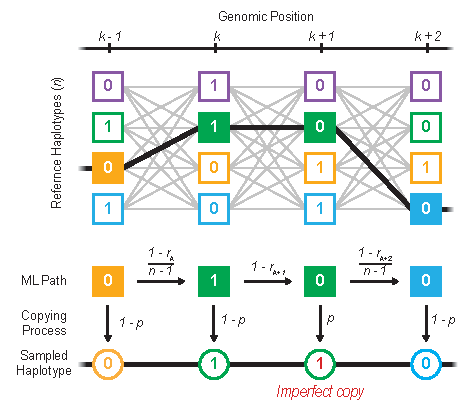
\includegraphics[width=0.99\linewidth]{Fig_B2.pdf}
\captionof{figure}{
\footnotesize{\textbf{Schematic representation of Li and Stephens hidden Markov model}. A new haplotype can be sampled as an imperfect copy of n reference haplotypes (hidden states). To find the most likely path taken through the hidden states, the LS model works along the genome (k-1, k, k+1, …), calculating the probabilities of changes in the attributed haplotype. The transition probability to continue or switch the attributed haplotype is a function of the recombination rate (r) between adjacent sites, whilst the emission probability to copy the attributed allele with or without error is a function of the mutation rate (p). Moving along the genome, the LS model compares the probability of every possible copying path and infers the most likely one.}
    \label{fig:B2}}
    
\end{multicols}
\end{tcolorbox}
\end{strip}

\section*{Conclusions and future directions}
In this article, we have outlined a definition of the haplotype block as an edge on the ARG, explored the implications of the definition with simple simulations, and considered how current methods can infer such blocks from empirical data. In our view, haplotypes and haplotype blocks should be the core concepts through which we understand population genetic processes. Under this view, it follows that ideally, genomic datasets should come directly as resolved haplotypes, rather than diploid genotypes that require phasing and further processing. We therefore welcome new developments in linked- and long-read sequencing techniques, analysis software, and visualization tools that are designed with sequencing and population datasets in mind (Davies et al., 2021; Meier et al., 2021).

Our simulations and empirical example show that haplotype blocks contain rich information about the demographic and selective history of the locus. Making the most of this information will require a fundamental rethink of our linear, reference-based genome assemblies, and a move towards a graph, or tree-based assembly standard to take advantage of their capability to natively encode variation (Eggertsson et al., 2017; Hickey et al., 2020). We will also need new concepts and vocabulary to describe features in these graphs (e.g., super-graphs and “bubbles”; (Cheng et al., 2021; Turner et al., 2018; Weisenfeld et al., 2017) informed by a robust understanding of the generative process discussed above, and we need to align our mental models with inference schemes and their encoding (as in, e.g., tsinfer). For that reason, we hope our discussion here can focus our effort towards this new standard, as haplotype-resolved sequencing becomes routine.

\phantom{\cite{}}



%%%%%%%%%%%%%%%%%%%%%%%%%%%%%%%%%%%%%%%%%%%%%%
%%                                          %%
%% Backmatter begins here                   %%
%%                                          %%
%%%%%%%%%%%%%%%%%%%%%%%%%%%%%%%%%%%%%%%%%%%%%%

\begin{backmatter}

\section*{Acknowledgements}%% if any
We thank the Barton group for useful discussion and feedback during the writing of this article. Comments from Roger Butlin, Molly Schumer’s Group, the tskit development team, editors and three reviewers greatly improved the manuscript. Funding was provided by SCAS (Natural Sciences Programme, Knut and Alice Wallenberg Foundation), an FWF Wittgenstein grant (PT1001Z211), an FWF standalone grant (grant P 32166), and an ERC Advanced Grant. YFC was supported by the Max Planck Society and an ERC Proof of Concept Grant \#101069216 (HAPLOTAGGING). 

\section*{Availability of data}%% if any
The mathematics notebook used to generate supplement 1 is available on dryad under the accession number xxxx. The \textit{Heliconius} sequence data was previously deposited at the National Center for Biotechnology Information Sequence Read Archive under the BioProject accession number PRJNA670070.

\section*{Authors' contributions}
All authors conceived the ideas and contributed to the writing of the manuscript. NHB conducted the simulations and AP implemented practical example.

\section*{ORCID}
DS: \url{http://orcid.org/0000-0002-1145-9226} \\
SS: \url{http://orcid.org/ 0000-0003-0472-9299} \\
AP: \url{http://orcid.org/0000-0002-4530-8469} \\
YFC: \url{http://orcid.org/0000-0001-6292-9681} \\
NHB: \url{http://orcid.org/0000-0002-8548-5240}


\begin{thebibliography}{xx}

\end{thebibliography}

%\section*{References}

\begin{hangparas}{1em}{1}

Al Bkhetan, Z., Zobel, J., Kowalczyk, A., Verspoor, K., \& Goudey, B.
(2019). Exploring effective approaches for haplotype block phasing.
\emph{BMC Bioinformatics}, \emph{20}(1), 540.

Berg, J. J., Harpak, A., Sinnott-Armstrong, N., Joergensen, A. M.,
Mostafavi, H., Field, Y., Boyle, E. A., Zhang, X., Racimo, F.,
Pritchard, J. K., \& Coop, G. (2019). Reduced signal for polygenic
adaptation of height in UK Biobank. \emph{ELife}, \emph{8}.
https://doi.org/10.7554/eLife.39725

Bhat, J. A., Yu, D., Bohra, A., Ganie, S. A., \& Varshney, R. K. (2021).
Features and applications of haplotypes in crop breeding.
\emph{Communications Biology}, \emph{4}(1), 1--12.

Brandt, D. Y. C., Wei, X., Deng, Y., Vaughn, A. H., \& Nielsen, R.
(2021). Evaluation of methods for the inference of ancestral
recombination graphs. In \emph{bioRxiv} (p. 2021.11.15.468686).
https://doi.org/10.1101/2021.11.15.468686

Browning, B. L., \& Browning, S. R. (2009). A unified approach to
genotype imputation and haplotype-phase inference for large data sets of
trios and unrelated individuals. \emph{American Journal of Human
Genetics}, \emph{84}(2), 210--223.

Browning, B. L., \& Browning, S. R. (2013). Improving the accuracy and
efficiency of identity-by-descent detection in population data.
\emph{Genetics}, \emph{194}(2), 459--471.

Browning, S. R., \& Browning, B. L. (2007). Rapid and accurate haplotype
phasing and missing-data inference for whole-genome association studies
by use of localized haplotype clustering. \emph{American Journal of
Human Genetics}, \emph{81}(5), 1084--1097.

Browning, S. R., \& Browning, B. L. (2011). Haplotype phasing: existing
methods and new developments. \emph{Nature Reviews. Genetics},
\emph{12}(10), 703--714.

Burri, R. (2017). Interpreting differentiation landscapes in the light
of long‐term linked selection. \emph{Evolution Letters}.
https://onlinelibrary.wiley.com/doi/abs/10.1002/evl3.14

Cao, J., Schneeberger, K., Ossowski, S., Günther, T., Bender, S., Fitz,
J., Koenig, D., Lanz, C., Stegle, O., Lippert, C., Wang, X., Ott, F.,
Müller, J., Alonso-Blanco, C., Borgwardt, K., Schmid, K. J., \& Weigel,
D. (2011). Whole-genome sequencing of multiple Arabidopsis thaliana
populations. \emph{Nature Genetics}, \emph{43}(10), 956--963.

Carmi, S., Palamara, P. F., Vacic, V., Lencz, T., Darvasi, A., \& Pe'er,
I. (2013). The Variance of Identity-by-Descent Sharing in the
Wright--Fisher Model. \emph{Genetics}, \emph{193}(3), 911--928.

Castro, J. P. L., Yancoskie, M. N., Marchini, M., Belohlavy, S.,
Hiramatsu, L., Kučka, M., Beluch, W. H., Naumann, R., Skuplik, I., Cobb,
J., Barton, N. H., Rolian, C., \& Chan, Y. F. (2019). An integrative
genomic analysis of the Longshanks selection experiment for longer limbs
in mice. \emph{ELife}, \emph{8}, e42014.

Cheng, H., Concepcion, G. T., Feng, X., Zhang, H., \& Li, H. (2021).
Haplotype-resolved de novo assembly using phased assembly graphs with
hifiasm. \emph{Nature Methods}, \emph{18}(2), 170--175.

Clark, A. G. (2004). The role of haplotypes in candidate gene studies.
\emph{Genetic Epidemiology}, \emph{27}(4), 321--333.

Crawford, D. C., \& Nickerson, D. A. (2005). Definition and clinical
importance of haplotypes. \emph{Annual Review of Medicine}, 56,
303--320.

Davies, R. W., Flint, J., Myers, S., \& Mott, R. (2016). Rapid genotype
imputation from sequence without reference panels. \emph{Nature
Genetics}, \emph{48}(8), 965--969.

Davies, R. W., Kucka, M., Su, D., Shi, S., Flanagan, M., Cunniff, C. M.,
Chan, Y. F., \& Myers, S. (2021). Rapid genotype imputation from
sequence with reference panels. \emph{Nature Genetics}, \emph{53}(7),
1104--1111.

Delaneau, O., Zagury, J.-F., Robinson, M. R., Marchini, J. L., \&
Dermitzakis, E. T. (2019). Accurate, scalable and integrative haplotype
estimation. \emph{Nature Communications}, 10(1), 5436.

Eggertsson, H. P., Jonsson, H., Kristmundsdottir, S., Hjartarson, E.,
Kehr, B., Masson, G., Zink, F., Hjorleifsson, K. E., Jonasdottir, A.,
Jonasdottir, A., Jonsdottir, I., Gudbjartsson, D. F., Melsted, P.,
Stefansson, K., \& Halldorsson, B. V. (2017). Graphtyper enables
population-scale genotyping using pangenome graphs. \emph{Nature
Genetics}, 49(11), 1654--1660.

Fisher, R. A. (1954). A fuller theory of ``Junctions'' in inbreeding.
\emph{Heredity}, \emph{8}(2), 187--197.

Griffiths, R. C., \& Marjoram, P. (1997). An ancestral recombination
graph. \emph{Institute for Mathematics and Its Applications}, \emph{87},
257.

Grossman, S. R., Shylakhter, I., Karlsson, E. K., Byrne, E. H., Morales,
S., Frieden, G., Hostetter, E., Angelino, E., Garber, M., Zuk, O.,
Lander, E. S., Schaffner, S. F., \& Sabeti, P. C. (2010). A Composite of
Multiple Signals Distinguishes Causal Variants in Regions of Positive
Selection. \emph{Science}, \emph{327}(5967), 883--886.

Hartl, D. L., Clark, A. G., \& Clark, A. G. (1997). \emph{Principles of
population genetics} (Vol. 116). Sinauer associates Sunderland, MA.

Hellenthal, G., Busby, G. B. J., Band, G., Wilson, J. F., Capelli, C.,
Falush, D., \& Myers, S. (2014). A genetic atlas of human admixture
history. \emph{Science}, \emph{343}(6172), 747--751.

Hickey, G., Heller, D., Monlong, J., Sibbesen, J. A., Sirén, J.,
Eizenga, J., Dawson, E. T., Garrison, E., Novak, A. M., \& Paten, B.
(2020). Genotyping structural variants in pangenome graphs using the vg
toolkit. \emph{Genome Biology}, \emph{21}(1), 35.

Howie, B., Marchini, J., \& Stephens, M. (2011). Genotype imputation
with thousands of genomes. \emph{G3} , \emph{1}(6), 457--470.

Howie, B. N., Donnelly, P., \& Marchini, J. (2009). A flexible and
accurate genotype imputation method for the next generation of
genome-wide association studies. \emph{PLoS Genetics}, \emph{5}(6),
e1000529.

Hubisz, M. J., Williams, A. L., \& Siepel, A. (2020). Mapping gene flow
between ancient hominins through demography-aware inference of the
ancestral recombination graph. \emph{PLoS Genetics}, \emph{16}(8),
e1008895.

Hudson, R. R. (1983). Properties of a neutral allele model with
intragenic recombination. \emph{Theoretical Population Biology},
\emph{23}(2), 183--201.

Hudson, Richard R. (1990). Gene genealogies and the coalescent process.
\emph{Oxford Surveys in Evolutionary Biology}, \emph{7}(1), 44.

International HapMap Consortium. (2005). A haplotype map of the human
genome. \emph{Nature}, \emph{437}(7063), 1299--1320.

Jones, F. C., Grabherr, M. G., Chan, Y. F., Russell, P., Mauceli, E.,
Johnson, J., Swofford, R., Pirun, M., Zody, M. C., White, S., Birney,
E., Searle, S., Schmutz, J., Grimwood, J., Dickson, M. C., Myers, R. M.,
Miller, C. T., Summers, B. R., Knecht, A. K., \ldots{} Kingsley, D. M.
(2012). The genomic basis of adaptive evolution in threespine
sticklebacks. \emph{Nature}, \emph{484}(7392), 55--61.

Kelleher, J., Wong, Y., Wohns, A. W., Fadil, C., Albers, P. K., \&
McVean, G. (2019). Inferring whole-genome histories in large population
datasets. \emph{Nature Genetics}, \emph{51}(9), 1330--1338.

Kingman, J. F. C. (1982). The coalescent. \emph{Stochastic Processes and
Their Applications}, \emph{13}(3), 235--248.

Lawson, D. J., Hellenthal, G., Myers, S., \& Falush, D. (2012).
Inference of population structure using dense haplotype data. \emph{PLoS
Genetics}, \emph{8}(1), e1002453.

Leitwein, M., Duranton, M., Rougemont, Q., Gagnaire, P.-A., \&
Bernatchez, L. (2020). Using Haplotype Information for Conservation
Genomics. \emph{Trends in Ecology \& Evolution}, \emph{35}(3), 245--258.

Lewis, J.J., Geltman, R.C., Pollak, P.C., Rondem, K.E., Van Belleghem,
S.M., Hubisz, M.J., Munn, P.R., Zhang, L., Benson, C., Mazo-Vargas, A.
and Danko, C.G., 2019. Parallel evolution of ancient, pleiotropic
enhancers underlies butterfly wing pattern mimicry. \emph{Proceedings of
the National Academy of Sciences}, 116(48), pp.24174-24183.

Li, H., \& Ralph, P. (2019). Local PCA Shows How the Effect of
Population Structure Differs Along the Genome. \emph{Genetics},
\emph{211}(1), 289--304.

Li, N., \& Stephens, M. (2003). Modeling linkage disequilibrium and
identifying recombination hotspots using single-nucleotide polymorphism
data. \emph{Genetics}, \emph{165}(4), 2213--2233.

Li, Y., Willer, C. J., Ding, J., Scheet, P., \& Abecasis, G. R. (2010).
MaCH: using sequence and genotype data to estimate haplotypes and
unobserved genotypes. \emph{Genetic Epidemiology}, \emph{34}(8),
816--834.

Lohse, K., Chmelik, M., Martin, S. H., \& Barton, N. H. (2016).
Efficient Strategies for Calculating Blockwise Likelihoods Under the
Coalescent. \emph{Genetics}, \emph{202}(2), 775--786.

Lundberg, M., Liedvogel, M., Larson, K., Sigeman, H., Grahn, M., Wright,
A., Åkesson, S., \& Bensch, S. (2017). Genetic differences between
willow warbler migratory phenotypes are few and cluster in large
haplotype blocks. Evolution Letters, \emph{1}(3), 155--168.

Marchini, J., Howie, B., Myers, S., McVean, G., \& Donnelly, P. (2007).
A new multipoint method for genome-wide association studies by
imputation of genotypes. \emph{Nature Genetics}, \emph{39}(7), 906--913.

Martin, S. H., \& Van Belleghem, S. M. (2017). Exploring Evolutionary
Relationships Across the Genome Using Topology Weighting.
\emph{Genetics}, \emph{206}(1), 429--438.

Maynard Smith, J. M., \& Haigh, J. (1974). The hitch-hiking effect of a
favourable gene. \emph{Genetical Research}, \emph{23}(1), 23--35.

McVean, G. A. T., \& Cardin, N. J. (2005). Approximating the coalescent
with recombination. \emph{Philosophical Transactions of the Royal
Society of London. Series B, Biological Sciences}, \emph{360}(1459),
1387--1393.

Meier, J. I., Salazar, P. A., Kučka, M., Davies, R. W., Dréau, A.,
Aldás, I., Box Power, O., Nadeau, N. J., Bridle, J. R., Rolian, C.,
Barton, N. H., McMillan, W. O., Jiggins, C. D., \& Chan, Y. F. (2021).
Haplotype tagging reveals parallel formation of hybrid races in two
butterfly species. \emph{Proceedings of the National Academy of Sciences
of the United States of America}, \emph{118}(25).
https://doi.org/10.1073/pnas.2015005118

Mészáros, G., Milanesi, M., Ajmone-Marsan, P., \& Utsunomiya, Y. T.
(2021). Editorial: Haplotype analysis applied to livestock genomics.
\emph{Frontiers in Genetics}, \emph{12}, 660478.

Novembre, J., \& Barton, N. H. (2018). Tread Lightly Interpreting
Polygenic Tests of Selection. \emph{Genetics}, \emph{208}(4),
1351--1355.

Otte, K. A., \& Schlötterer, C. (2021). Detecting selected haplotype
blocks in evolve and resequence experiments. \emph{Molecular Ecology
Resources}, \emph{21}(1), 93--109.

Patil, N., Berno, A. J., Hinds, D. A., Barrett, W. A., Doshi, J. M.,
Hacker, C. R., Kautzer, C. R., Lee, D. H., Marjoribanks, C., McDonough,
D. P., Nguyen, B. T., Norris, M. C., Sheehan, J. B., Shen, N., Stern,
D., Stokowski, R. P., Thomas, D. J., Trulson, M. O., Vyas, K. R.,
\ldots{} Cox, D. R. (2001). Blocks of limited haplotype diversity
revealed by high-resolution scanning of human chromosome 21.
\emph{Science}, \emph{294}(5547), 1719--1723.

Poelstra, J. W., Vijay, N., Bossu, C. M., Lantz, H., Ryll, B., Müller,
I., Baglione, V., Unneberg, P., Wikelski, M., Grabherr, M. G., \& Wolf,
J. B. W. (2014). The genomic landscape underlying phenotypic integrity
in the face of gene flow in crows. \emph{Science}, \emph{344}(6190),
1410--1414.

Price, A. L., Tandon, A., Patterson, N., Barnes, K. C., Rafaels, N.,
Ruczinski, I., Beaty, T. H., Mathias, R., Reich, D., \& Myers, S.
(2009). Sensitive detection of chromosomal segments of distinct ancestry
in admixed populations. \emph{PLoS Genetics}, \emph{5}(6), e1000519.

Ralph, P., Thornton, K., \& Kelleher, J. (2020). Efficiently Summarizing
Relationships in Large Samples: A General Duality Between Statistics of
Genealogies and Genomes. \emph{Genetics}, \emph{215}(3), 779--797.

Rasmussen, M. D., Hubisz, M. J., Gronau, I., \& Siepel, A. (2014).
Genome-wide inference of ancestral recombination graphs. \emph{PLoS
Genetics}, \emph{10}(5), e1004342.

Ravinet, M., Faria, R., Butlin, R. K., Galindo, J., Bierne, N.,
Rafajlović, M., Noor, M. A. F., Mehlig, B., \& Westram, A. M. (2017).
Interpreting the genomic landscape of speciation: a road map for finding
barriers to gene flow. \emph{Journal of Evolutionary Biology},
\emph{30}(8), 1450--1477.

Richardson, J. L., Brady, S. P., Wang, I. J., \& Spear, S. F. (2016).
Navigating the pitfalls and promise of landscape genetics.
\emph{Molecular Ecology}, \emph{25}(4), 849--863.

Rockman, M. V. (2012). The QTN program and the alleles that matter for
evolution: all that's gold does not glitter. \emph{Evolution;
International Journal of Organic Evolution}, \emph{66}(1), 1--17.

Sabeti, P. C., Reich, D. E., Higgins, J. M., Levine, H. Z. P., Richter,
D. J., Schaffner, S. F., Gabriel, S. B., Platko, J. V., Patterson, N.
J., McDonald, G. J., Ackerman, H. C., Campbell, S. J., Altshuler, D.,
Cooper, R., Kwiatkowski, D., Ward, R., \& Lander, E. S. (2002).
Detecting recent positive selection in the human genome from haplotype
structure. \emph{Nature}, \emph{419}(6909), 832--837.

Sabeti, P. C., Varilly, P., Fry, B., Lohmueller, J., Hostetter, E.,
Cotsapas, C., Xie, X., Byrne, E. H., McCarroll, S. A., Gaudet, R.,
Schaffner, S. F., Lander, E. S., International HapMap Consortium,
Frazer, K. A., Ballinger, D. G., Cox, D. R., Hinds, D. A., Stuve, L. L.,
Gibbs, R. A., \ldots{} Stewart, J. (2007). Genome-wide detection and
characterization of positive selection in human populations.
\emph{Nature}, \emph{449}(7164), 913--918.

Schwartz, R., Halldórsson, B. V., Bafna, V., Clark, A. G., \& Istrail,
S. (2003). Robustness of inference of haplotype block structure.
\emph{Journal of Computational Biology: A Journal of Computational
Molecular Cell Biology}, \emph{10}(1), 13--19.

Sella, G., \& Barton, N. H. (2019). Thinking About the Evolution of
Complex Traits in the Era of Genome-Wide Association Studies.
\emph{Annual Review of Genomics and Human Genetics}, \emph{20},
461--493.

Sousa, V. C., Grelaud, A., \& Hey, J. (2011). On the nonidentifiability
of migration time estimates in isolation with migration models.
\emph{Molecular Ecology}, \emph{20}(19), 3956--3962.

Speidel, L., Forest, M., Shi, S., \& Myers, S. R. (2019). A method for
genome-wide genealogy estimation for thousands of samples. \emph{Nature
Genetics}, \emph{51}(9), 1321--1329.

Stankowski, S., Chase, M. A., Fuiten, A. M., Rodrigues, M. F., Ralph, P.
L., \& Streisfeld, M. A. (2019). Widespread selection and gene flow
shape the genomic landscape during a radiation of monkeyflowers.
\emph{PLoS Biology}, \emph{17}(7), e3000391.

Stankowski, S., \& Streisfeld, M. A. (2015). Introgressive hybridization
facilitates adaptive divergence in a recent radiation of monkeyflowers.
\emph{Proceedings. Biological Sciences / The Royal Society},
\emph{282}(1814). https://doi.org/10.1098/rspb.2015.1666

Steinrücken, M., Kamm, J., Spence, J. P., \& Song, Y. S. (2019).
Inference of complex population histories using whole-genome sequences
from multiple populations. \emph{Proceedings of the National Academy of
Sciences of the United States of America}, \emph{116}(34), 17115--17120.

Steinrücken, M., Spence, J. P., Kamm, J. A., Wieczorek, E., \& Song, Y.
S. (2018). Model-based detection and analysis of introgressed
Neanderthal ancestry in modern humans. \emph{Molecular Ecology},
\emph{27}(19), 3873--3888.

Stephens, M., \& Scheet, P. (2005). Accounting for decay of linkage
disequilibrium in haplotype inference and missing-data imputation.
\emph{American Journal of Human Genetics}, \emph{76}(3), 449--462.

Sundquist, A., Fratkin, E., Do, C. B., \& Batzoglou, S. (2008). Effect
of genetic divergence in identifying ancestral origin using HAPAA.
\emph{Genome Research}, \emph{18}(4), 676--682.

Szpiech, Z. A., \& Hernandez, R. D. (2014). selscan: an efficient
multithreaded program to perform EHH-based scans for positive selection.
\emph{Molecular Biology and Evolution}, \emph{31}(10), 2824--2827.

Taliun, D., Gamper, J., \& Pattaro, C. (2014). Efficient haplotype block
recognition of very long and dense genetic sequences. \emph{BMC
Bioinformatics}, \emph{15}, 10.

Tavares, H., Whibley, A., Field, D. L., Bradley, D., Couchman, M.,
Copsey, L., Elleouet, J., Burrus, M., Andalo, C., Li, M., Li, Q., Xue,
Y., Rebocho, A. B., Barton, N. H., \& Coen, E. (2018). Selection and
gene flow shape genomic islands that control floral guides.
\emph{Proceedings of the National Academy of Sciences of the United
States of America}, \emph{115}(43), 11006--11011.

Thompson, E. A. (2013). Identity by descent: variation in meiosis,
across genomes, and in populations. \emph{Genetics}, \emph{194}(2),
301--326.

Todesco, M., Owens, G. L., Bercovich, N., Légaré, J.-S., Soudi, S.,
Burge, D. O., Huang, K., Ostevik, K. L., Drummond, E. B. M., Imerovski,
I., Lande, K., Pascual-Robles, M. A., Nanavati, M., Jahani, M., Cheung,
W., Staton, S. E., Muños, S., Nielsen, R., Donovan, L. A., \ldots{}
Rieseberg, L. H. (2020). Massive haplotypes underlie ecotypic
differentiation in sunflowers. \emph{Nature}, \emph{584}(7822),
602--607.

Turner, I., Garimella, K. V., Iqbal, Z., \& McVean, G. (2018).
Integrating long-range connectivity information into de Bruijn graphs.
\emph{Bioinformatics} , \emph{34}(15), 2556--2565.

Voight, B. F., Kudaravalli, S., Wen, X., \& Pritchard, J. K. (2006). A
map of recent positive selection in the human genome. \emph{PLoS
Biology}, \emph{4}(3), e72.

Wallbank, W. R., Baxter S.W., Pardo-Diaz, C., Hanly, J. J., Martin, S.
H., Mallet, J., Dasmahapatra, K.K., et al. (2016) "Evolutionary novelty
in a butterfly wing pattern through enhancer shuffling." \emph{PLoS
biology} 14: e1002353.

Wakeley, J. (2009). \emph{Coalescent theory :an introduction /}
(575:519.2 WAK). 

Wakeley, J., \& Wilton, P. R. (2016). \emph{Coalescent and models of
identity by descent}.

Wallberg, A., Schöning, C., Webster, M. T., \& Hasselmann, M. (2017).
Two extended haplotype blocks are associated with adaptation to high
altitude habitats in East African honey bees. \emph{PLoS Genetics},
\emph{13}(5), e1006792.

Weisenfeld, N. I., Kumar, V., Shah, P., Church, D. M., \& Jaffe, D. B.
(2017). Direct determination of diploid genome sequences. \emph{Genome
Research}, \emph{27}(5), 757--767.

Whitlock, M. C., \& Mccauley, D. E. (1999). Indirect measures of gene
flow and migration: FST/=1/(4Nm+1). \emph{Heredity}, \emph{82}(2),
117--125.

Wohns, A. W., Wong, Y., Jeffery, B., Akbari, A., Mallick, S., Pinhasi,
R., Patterson, N., Reich, D., Kelleher, J., \& McVean, G. (2021). A
unified genealogy of modern and ancient genomes. In \emph{bioRxiv} (p.
2021.02.16.431497). https://doi.org/10.1101/2021.02.16.431497

Wolf, J. B. W., \& Ellegren, H. (2017). Making sense of genomic islands
of differentiation in light of speciation. \emph{Nature Reviews.
Genetics}, \emph{18}(2), 87--100.

Zhang, K., Calabrese, P., Nordborg, M., \& Sun, F. (2002). Haplotype
block structure and its applications to association studies: power and
study designs. \emph{American Journal of Human Genetics}, \emph{71}(6),
1386--1394.

\end{hangparas}



%%%%%%%%%%%%%%%%%%%%%%%%%%%%%%%%%%%%%%%%%%%%%%%%%%%%%%%%%%%%%
%%                  The Bibliography                       %%
%%                                                         %%
%%  Bmc_mathpys.bst  will be used to                       %%
%%  create a .BBL file for submission.                     %%
%%  After submission of the .TEX file,                     %%
%%  you will be prompted to submit your .BBL file.         %%
%%                                                         %%
%%                                                         %%
%%  Note that the displayed Bibliography will not          %%
%%  necessarily be rendered by Latex exactly as specified  %%
%%  in the online Instructions for Authors.                %%
%%                                                         %%
%%%%%%%%%%%%%%%%%%%%%%%%%%%%%%%%%%%%%%%%%%%%%%%%%%%%%%%%%%%%%

% if your bibliography is in bibtex format, use those commands:
%\bibliographystyle{bmc-mathphys} % Style BST file (bmc-mathphys, vancouver, spbasic).
%\bibliography{bmc_article}      % Bibliography file (usually '*.bib' )
% for author-year bibliography (bmc-mathphys or spbasic)
% a) write to bib file (bmc-mathphys only)
% @settings{label, options="nameyear"}
% b) uncomment next line
%\nocite{label}

% or include bibliography directly:
% \begin{thebibliography}
% \bibitem{b1}
% \end{thebibliography}

%%%%%%%%%%%%%%%%%%%%%%%%%%%%%%%%%%%
%%                               %%
%% Figures                       %%
%%                               %%
%% NB: this is for captions and  %%
%% Titles. All graphics must be  %%
%% submitted separately and NOT  %%
%% included in the Tex document  %%
%%                               %%
%%%%%%%%%%%%%%%%%%%%%%%%%%%%%%%%%%%

%%
%% Do not use \listoffigures as most will included as separate files


%%%%%%%%%%%%%%%%%%%%%%%%%%%%%%%%%%%
%%                               %%
%% Tables                        %%
%%                               %%
%%%%%%%%%%%%%%%%%%%%%%%%%%%%%%%%%%%

%% Use of \listoftables is discouraged.
%%


%%%%%%%%%%%%%%%%%%%%%%%%%%%%%%%%%%%
%%                               %%
%% Additional Files              %%
%%                               %%
%%%%%%%%%%%%%%%%%%%%%%%%%%%%%%%%%%%



\end{backmatter}
%\bibliography{bmc_article}

\end{document}
